\documentclass[a4paper, 11pt]{report}
\usepackage[a4paper,margin=1in]{geometry}
\usepackage{dirtree}
 \usepackage[at]{easylist}
\usepackage[utf8]{inputenc}
\usepackage{graphicx}
\usepackage{hyperref}
\usepackage{fancyhdr}
\graphicspath{ {./Figures/} }
\usepackage[table,xcdraw]{xcolor}
\usepackage[export]{adjustbox}
\usepackage{listings}
\usepackage{xcolor}
\usepackage{float}
\usepackage{longtable}
\usepackage[normalem]{ulem}
\useunder{\uline}{\ul}{}
\usepackage{longtable}
\definecolor{codegreen}{rgb}{0,0.6,0}
\definecolor{codegray}{rgb}{0.5,0.5,0.5}
\definecolor{codepurple}{rgb}{0.58,0,0.82}
\definecolor{backcolour}{rgb}{0.95,0.95,0.92}
\setlength{\headheight}{13.6pt}
\newenvironment{simplechar}{%
   \catcode`\$=12
   \catcode`\&=12
   \catcode`\#=12
   \catcode`\^=12
   \catcode`\_=12
   \catcode`\~=12
   \catcode`\%=12
}{}

\lstdefinestyle{mystyle}{
    backgroundcolor=\color{backcolour},   
    commentstyle=\color{codegreen},
    keywordstyle=\color{magenta},
    numberstyle=\tiny\color{codegray},
    stringstyle=\color{codepurple},
    basicstyle=\ttfamily\footnotesize,
    breakatwhitespace=false,         
    breaklines=true,                 
    captionpos=b,                    
    keepspaces=true,                 
     numbers=left,                    
    numbersep=5pt,                  
    showspaces=false,                
    showstringspaces=false,
    showtabs=false,                  
    tabsize=2
}

\lstset{style=mystyle}

\definecolor{codegreen}{rgb}{0,0.6,0}
\definecolor{codegray}{rgb}{0.5,0.5,0.5}
\definecolor{codepurple}{HTML}{C42043}
\definecolor{backcolour}{HTML}{F2F2F2}
\definecolor{bookColor}{cmyk}{0,0,0,0.90}  
\color{bookColor}

\lstset{upquote=true}

\lstdefinestyle{mystyle1}{
    backgroundcolor=\color{backcolour},   
    commentstyle=\color{codegreen},
    keywordstyle=\color{codepurple},
    numberstyle=\numberstyle,
    stringstyle=\color{codepurple},
    basicstyle=\footnotesize\ttfamily,
    breakatwhitespace=false,
    breaklines=true,
    captionpos=b,
    keepspaces=true,
    numbers=left,
    numbersep=10pt,
    showspaces=false,
    showstringspaces=false,
    showtabs=false,
}

\fancypagestyle{plain}{
  \fancyhf{}% Clear header/footer
  \rhead{John Montgomery - 5199}
\lhead{Kimberley College - 15162}
\lfoot{\thepage}
\rfoot{Robotron 2084: Pygame remake}
}
\pagestyle{plain}% Set page style to plain.

\title{%
    
    \begin{center}
        
\includegraphics[width=3cm]{kimberley.png}
        \centering
    \end{center}
  Robotron: 2084 inspired Game \\
  \large Written in PyGame with MVC architecture}
\author{{\Large John Montgomery}\\ \ 
Candidate Number: 5199\\
Centre Name: Kimberley College\\
Centre Number: 15162\\
Qualification: AQA 7517 (A--Level Computer Science)\\ \\
{\small Supervisor: B. Harris}}
\date{2020-2022}




\begin{document}

\maketitle

\newpage
\tableofcontents\thispagestyle{empty}
\newpage
\listoffigures\thispagestyle{empty}
\newpage
\chapter{Abstract}
    This project is a modernised version of robotron 2084, it has 2 sections, the game code and the website. The game code, which is a remake of Robotron 2084, a classic arcade game, this is backed with an MVC architecture which is designed to separate out the functionalities of the game and communicates with the website via an API. The website will use a database with multiple tables to store all the scores and logins and will also be used to display the high scores of users.

\chapter{Analysis}
    \section{Introduction}
The goal of this project was to create a more modernised version of Robotron: 2084, the classic arcade game from the 80s. In order to make it a more modern version I will make a few additions, including improving the game itself and increase the competition aspect of it. I also needed to modernise the codebase itself, and couldnt build off the existing code written in the 80s.

As i was unable to access the code from the original game, nor find a viable method to emulate the code on my machine, i was forced to take my research from websites, videos and images, and whilst this isnt ideal, i was still able to gain a vast amount of information and replicate the game how i wanted to.

Whilst there is no specific target audience for the project, it could be played and enjoyed by anyone, ranging from my classmates to the people who played and enjoyed the original game from the 80s. Thanks to the wide range of possible users, there is a large market i can test this app with.

\section{About the game}

Robotron 2084 is a classic, top down, arcade game from the 80's, in which, a player (who is a mutant genetic super hero) attempts to save the last human family from swarms of killer robots. The game was a 2 stick shooter originally - this means 2 joysticks, one to move and one to shoot (this allows the 2 to occur individually and simultaneously). This was one of the first of its kind, and was largely considered a success. The game has a number of waves with varying number or robots, of different types, and varying numbers of humans.

In order to 'save' a human, they player simply has to touch them, this rescues the human and scores the player points. The more humans saved, the higher the points. The player, whilst a mutant, is still susceptible to damage - and whilst there is no 'health' the player can be killed rather easily. The robots simply have to touch the player (or the player accidentally collide with them) and the player 'dies'. You start the game with 3 lives and slowly progress through the waves - a new wave starts when all of the grunts (one of the robots, see table below) are killed, or when the player dies. 
There are also various transition screens, including a boot screen, a testing screen and end screens. Along with these come a live counter, a score counter and flashing borders. The game is fast passed and bright, and graphically complex, with lots of colours and intense action. Making a game like this play as smoothly as they did at the time was truly an accomplishment.
The game even had sound! whilst it was only mono aural (no stereo) - this was still impressive, considering it was a game running on a 1MHz processor. They were able to develop this in a 2 man team over a period of 6 months. It was itself heavily influenced by a number of other games, including 'Berzerk' - a shooting game which players traverse a maze and shoot at enemies. However, this was a single stick shooter (with a button to fire) rather than a dual stick shooter.
The game had sequels but none were as successful as the original, and were never received as well. One even attempted a multiplayer system, where one would shoot and another would move, but this was not widely seen as a positive update.

\section{More Modern 2D games}
In order to bring this game into the 21st century, it will need more modernised features. For one, almost everyone plays games on computers, and as such, will need a 'dual stick' implementation. Almost every modern game uses WASD to move and arrows to shoot, but IJKL is also used to shoot. Other approaches to avoid seeming like a single stick shooter are using the mouse to control movement or shooting, or even ESDX and IJKM as move and shoot (this was the original set up for Robotron 2084 on apple products. 

\section{Robotron's Design}
I mostly used video for my research into robotrons design - this felt like the best way due to how fast the game changes, with fast animations and colour changes, something that cannot be captured easily in photo screenshots. I also relied on websites, also linked, for more technical information and this is where i was also able to learn lots of the history behind the game.


\begin{itemize}
    \item \url{https://www.youtube.com/watch?v=ccltMtkFBSI} - This video - impressive in itelf for the gameplay, gave me more of an insight into the feel of the past paced nature of the game, and whilst the quality isnt perfect, it gives some idea of the general layout of the screen and game
    
    \item \url{https://www.youtube.com/watch?v=aOVA2Axxfdk} - This video was much higher quality screen capture of the game, this is what allowed me to see animation and character design as well as have a very good understanding of what layouts looked like, and the general interface.
    
    \item \url{https://arcadeblogger.com/2020/06/27/the-development-of-robotron/} This was possibly my most used resource. Having insight into the development and original views of the game was very important, and this website alone would probably have been enough to implement it. 
\end{itemize}

Whilst i didn't want to build a carbon copy of the original, i did endeavour to create something as similar as i could without loosing too much of the fast paced nature of the game.


\section{Robotron Step by Step}
Robotron starts up with a pattern of random pixels, followed by a screen indicating that tests were successful (or, as it may be, unsuccessful), before finally transitioning to the start screen. This screen has the words Robotron, along with credits to the developer. It is very bright, and flashing. The game also has a high score board displaying at the end of every run (and i believe it would also display at times when the machine was not in game). When starting the game, it would show a level transition screen (bright rectangles would display from the centre of the screen moving out). A wave would then start. This would begin by displaying all character, but not allowing movement of enemies for a few moments (this is probably a design choice, a brief moment for the player to plan their first few movements, and analyse where they should head). The levels would then loop like this, with a transition showing between each.

To illustrate the game layout better, i have included a finite state machine of how the game would work, it can be found below in \ref{fig:Robotron FSM}.

\begin{figure}[ht!]
  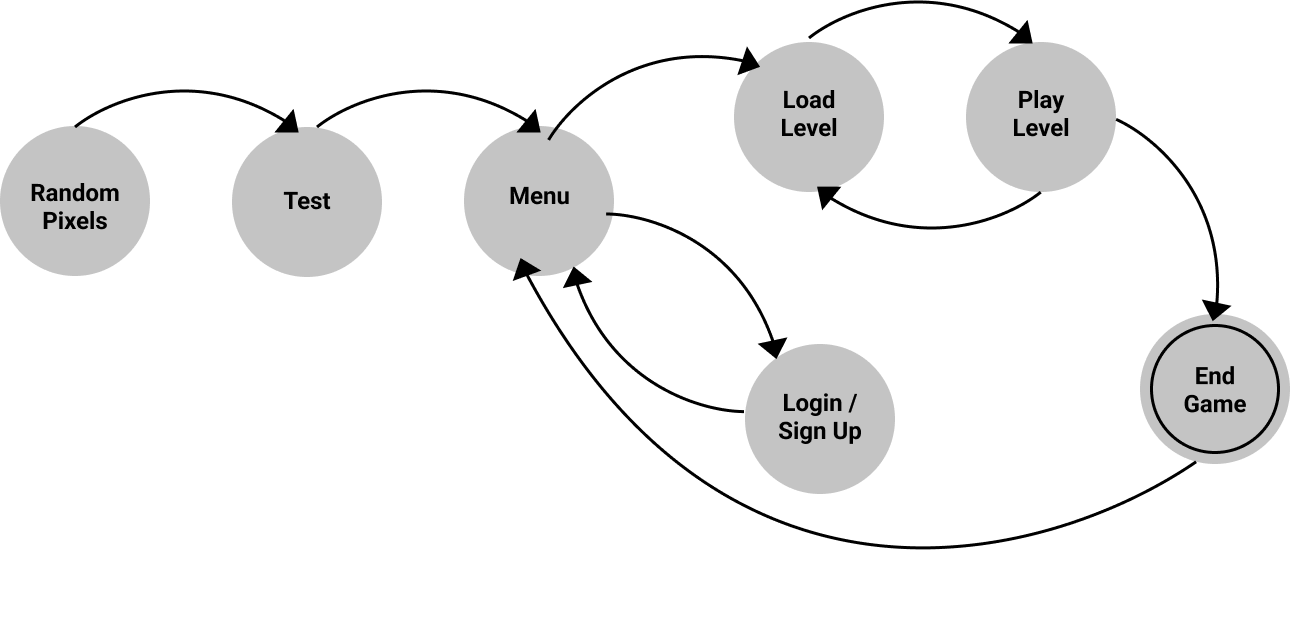
\includegraphics[width=0.8\linewidth]{Figures/FSM_robotrom.png}
  \centering
  \caption{The FSM which shows a very basic overview of how robotron 2084 works}
  \label{fig:Robotron_FSM}
\end{figure}


\section{Enemy Specific Behaviour}
One problem with not having access to the original code is the inability to tell what algorithm was used to cause the grunt enemy to 'flock' to the player (the only enemy I will implement which is actively seeking to get to the player) there are a few ways i could have done this, almost all of them much more simple than the method I would end up on.

A very basic approach to creating something like this is to simply move in the direction of the player, at a speed of x pixels per blit. This would have lead to some issues though. The main one being crowding. This would allow lots of grunts to 'stack', making it easier to kill them (a stream of bullets into this stack, and they are all destroyed). As such, this was rejected. I considered adding a random element to this (like having them move at a random speed, or adding some random direction) - but this would risk the grunts becoming jittery.

The solution is to use an algorithm called 'boids'. It is known as an artificial life program, and is meant to mimic the flocking of birds (boids = bird-oid object). It works by applying individual rules to each boid (each item in the flock) which results in a hive mind sort of intelligence. It is made up of 3 basic rules, plus 1 more to allow the group to move towards the goal (in this case the player).

\subsection{Rule 1 - move to centre mass}
First, calculate the centre of mass, for the boids in view. Essentially, sum all x and y co ordinate values and divide by the number of boids, for the co ordinates of the centre (c) $(\frac{\Sigma x}{n_{boids}},\frac{\Sigma y}{n_{boids}})$. Then, we want to move the boid 1\% of the way towards this centre, so our actual movement vector is given by $\frac{c - P_{boid}}{100}$ (where $P_{boid}$ is the position of the currently calculated boid), we need to subtract $P_{boid}$ as we want to move 1\% of the distance from the current position, not from the position $(0,0)$.
    
\subsection{Rule 2 - Avoid collisions with other boids}
This one is much more simple. For this, we simply want to move away from the other boids. To do that, just add the magnitudes of the difference between the 2 current positions to get a new position. 

\subsection{Rule 3 - Match velocities of the other boids}
This is also somewhat complex but works like Rule 1. We want to have the boids attempt to match the velocities of the boids around it. This could be done with some similar maths. First, sum all the velocities (V) $(\frac{\Sigma V_x}{n_{boids}},\frac{\Sigma V_y}{n_{boids}})$, much like with Rule 1, we dont want to match this velocty perfectly. Instead, add about a twentieth of the calculated value, which can be performed with $\frac{V - V_{boid}}{20}$

\subsection{Rule 4 - Move towards the player}
This rule is easy. Find the distance to the player, and move about a 5th of the way there.

\subsection{Notes on boids}
I did not create the boids flocking algorithm. It was created by Craig Reynolds, \url{http://www.red3d.com/cwr/boids/} is where i pulled most of my information from. This is a tweaked version from the original, with altered values that i set to perform more how i wanted (eg, to emulate a hoard of robots over flocking birds) and with the added rule of moving towards a player. 

\section{Python Library selection}
I had to select python libraries to handle 2 large sections of my code, these were the web framework and the gui framework. These both are hugely popular areas of python development, and there are a multitude of frameworks which i would have used, but there were 2 major contenders for each.

\subsection{Web Framework Library}
This was a relatively simple choice, flask or django. I had already decided that this would be a relatively simple website with a need for a larger focus to the API, and less need for web content. As such, django makes less sense, and flask is much faster, so this was quite an easy solution to use. In the past I've also found flask easier to deploy and debug, certainly it was my preference of backend anyway - but it also made sense.

\subsection{GUI Library}
Python has a few possible libraries, but again, 2 main contenders. TkInter and PyGame. TkInter is built in, and i have used it in the past, but when I used it, I used it for fairly basic forms, and at most, a chess game. These were no fast paced, and I wasnt convinced it would handle the huge number of sprites and fast moving objects. As such, I decided to go with Pygame, which is much better suited to this.

\section{Game Code Architecture}
Selecting an architecture was important. It was clear from the get go that this project would heavily use OOP, as it made sense, not just for sprites in general but also for its ease of use with pygame. I could have had a very simple system with a game loop and processing in there. I eventually settled on a specific design, and that was MVC (Model-View-Controller) as an architecture for the game.  This divides the logic into 3 components, 1, the model, which handles all the data, and is esentially the 'backend' of the game; 2, the view, this is the part the user sees, and is fed from the model, and finally, the controller, which is how the user interacts with the machine, and this feeds the model. 

For example, whilst it may have been possible to have it so that whenever a WASD key is pressed, the view is instantly moved to show the updated position - MVC dictates that you first update the model, and then on the next blit this update gets drawn up. This may seem somewhat counter intuative, but means each component can be swapped out much easier, leading to an incredibly modular design. This makes it much easier to develop, improve and test.

The system will also use a state machine (implemented with a stack) to control what is currently shown on screen as each state has its own meaning and definitions of what is needed on screen. Again, this allows for a much more modular system, as individual functions can be called once the current state is identified. It will also have an event system - such that it is a largely data driven system, where data is processed on the fly as it is received.

\section{Objectives}
\begin{easylist}[articletoc]
@ Game Objectives
@@ Main (hero) character objectives
@@@ Character can be displayed
@@@ Character can move in all 8 directions
@@@ Character faces in correct direction
@@@ Characters movement is animated
@@@ Character is bounded to window
@@@ Character can shoot in 8 directions
@@@ Player is invincible on load of level
@@ Enemy character objectives (for each enemy type - Electrodes, Grunts and Hunks)
@@@ Enemies can be displayed
@@@ Enemies can move
@@@ Enemy faces correct direction
@@@ Enemies movement is animated
@@@ Enemy are bounded to window
@@@ Enemy kills player when touching
@@@ Specific enemy functionality
@@@@ Electrodes are randomly spread around the page
@@@@ Grunts flock around player
@@@@ Hunks slow down when shot
@@ Menu objectives
@@@ Logo is shown and animated
@@@ Display static text
@@@ Display animated text
@@@ Display and allow input for options
@@@ Allow for login and sign up
@@ Extras objectives (additional features) 
@@@ Flashing border
@@@ Random colour load screen
@@@ "All tests" screen
@@@ Inter---level animation
@@@ Sounds
@@@@ For shooting
@@@@ For start up
@@@@ For level change

@ Website Objectives
@@ Displays high score board of top 10 players
@@ Website animated and looks like the high score board on original game
@@ Have an error page, informs user something went wrong
@@ API Goals (a route to...)
@@@ Return top scores
@@@ Allow for sign up
@@@ Allow for log in
@@@ Generate tokens for login
@@@ Upload scores and validate with token
\end{easylist}

\chapter{Documented Design}
    \section{Introduction}
This section will talk about all the design choices made in the creation of my Robotron inspired remake. This primarily includes a hierarchy chart, consisting of my objectives. However, it is important to note that this is more of a structure of how each objective interacts. The system interacts through MVC, and as such, i will also focus heavily (but in a different section) into the way in which MVC actually works, on a lower level, using pseudo code and diagrams to explain the entire system workings. This has been separated out of the hierarchy charts to avoid confusion.

\section{Hierarchy Charts}
The first chart sets the layout for the others. The chart had to be divided into smaller sections to allow for readability and easier implementation guidance. 

\begin{figure}[H]
  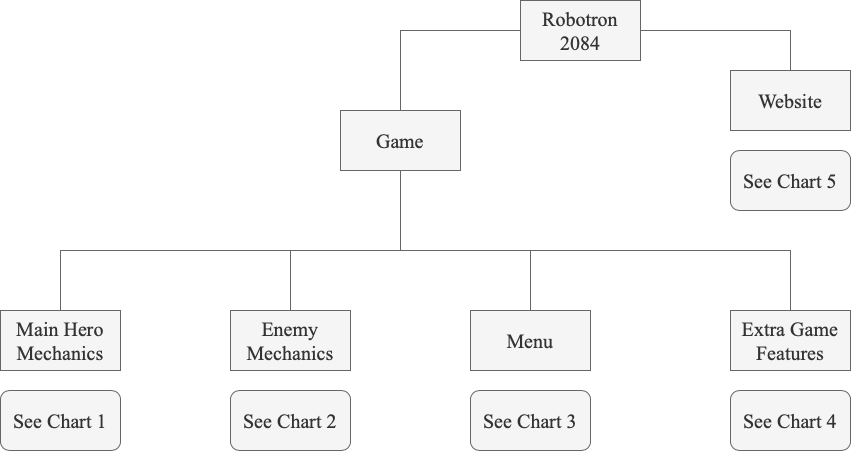
\includegraphics[width=0.8\linewidth]{Figures/chart0.png}
  \centering
  \caption{The first chart showing the basic overview}
  \label{fig:Chart_0}
\end{figure}

\begin{figure}[H]
  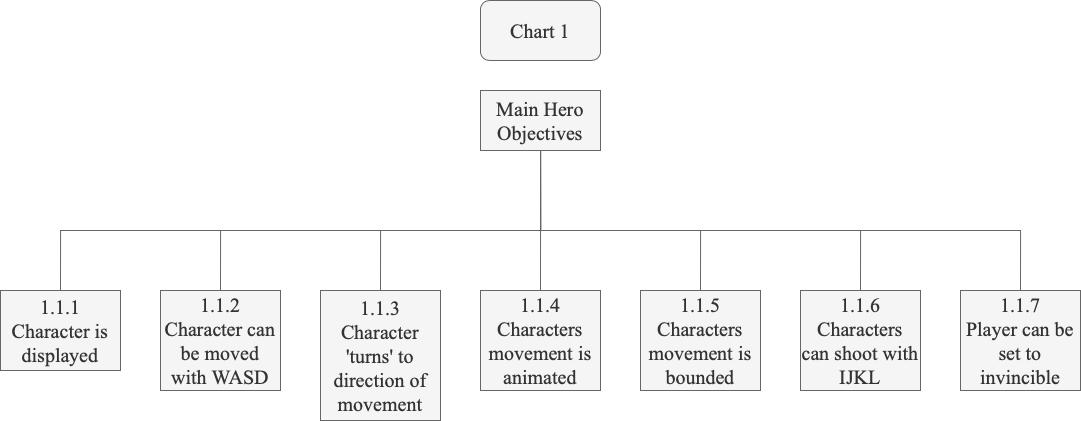
\includegraphics[width=1\linewidth]{Figures/chart1.png}
  \centering
  \caption{Chart detailing Main Hero Mechanics}
  \label{fig:Chart_1}
\end{figure}

\begin{figure}[H]
  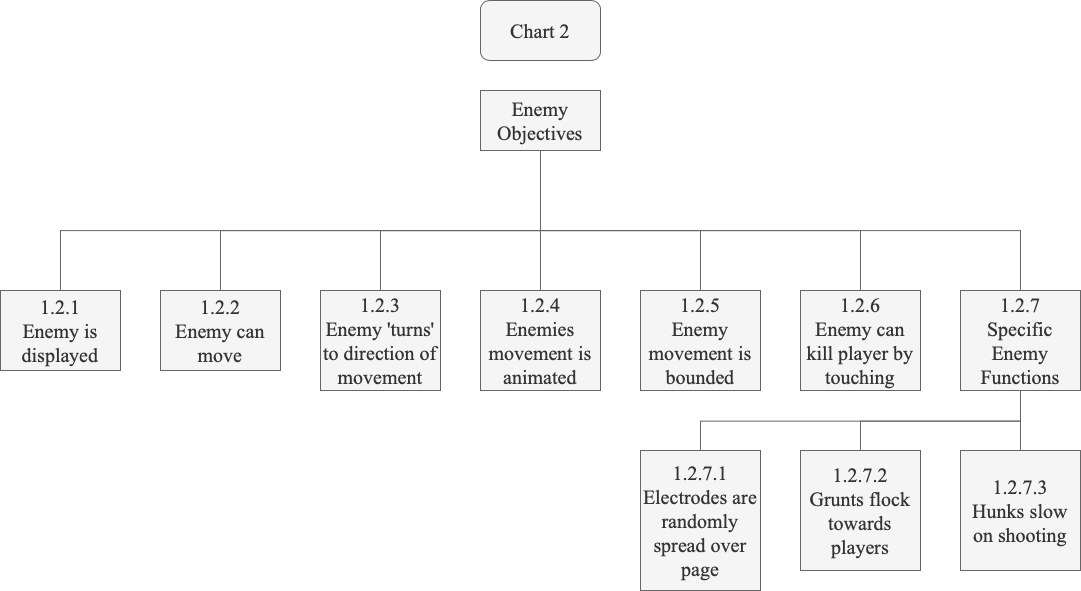
\includegraphics[width=1\linewidth]{Figures/chart2.png}
  \centering
  \caption{Chart detailing Enemy Mechanics}
  \label{fig:Chart_2}
\end{figure}

\begin{figure}[H]
  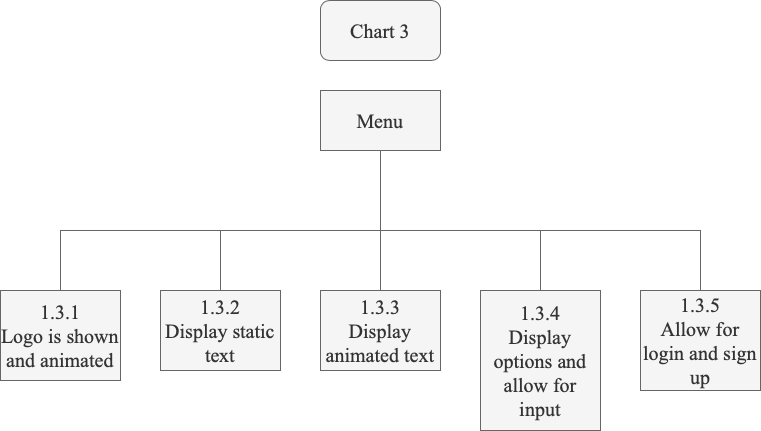
\includegraphics[width=0.6\linewidth]{Figures/chart3.png}
  \centering
  \caption{Chart detailing menu}
  \label{fig:Chart_3}
\end{figure}

\begin{figure}[H]
  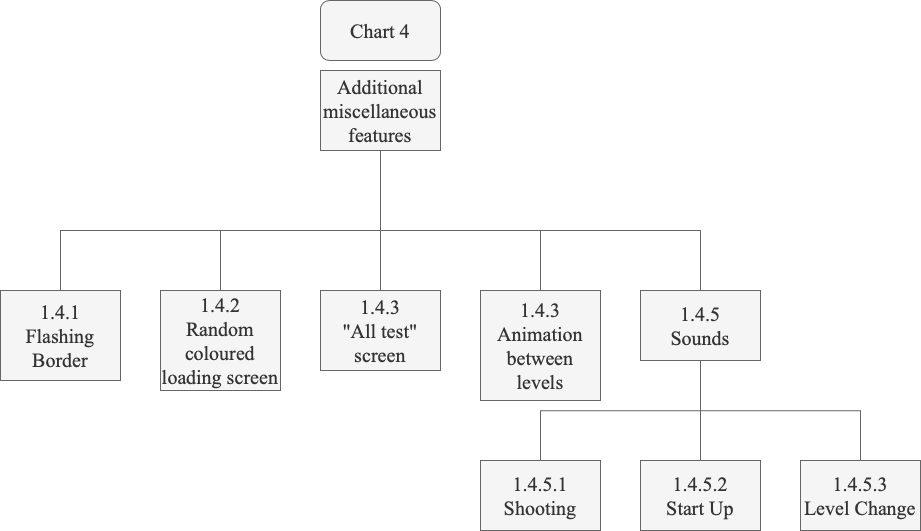
\includegraphics[width=1\linewidth]{Figures/chart4.png}
  \centering
  \caption{Chart detailing miscellaneous features}
  \label{fig:Chart_4}
  
\end{figure}
\begin{figure}[H]
  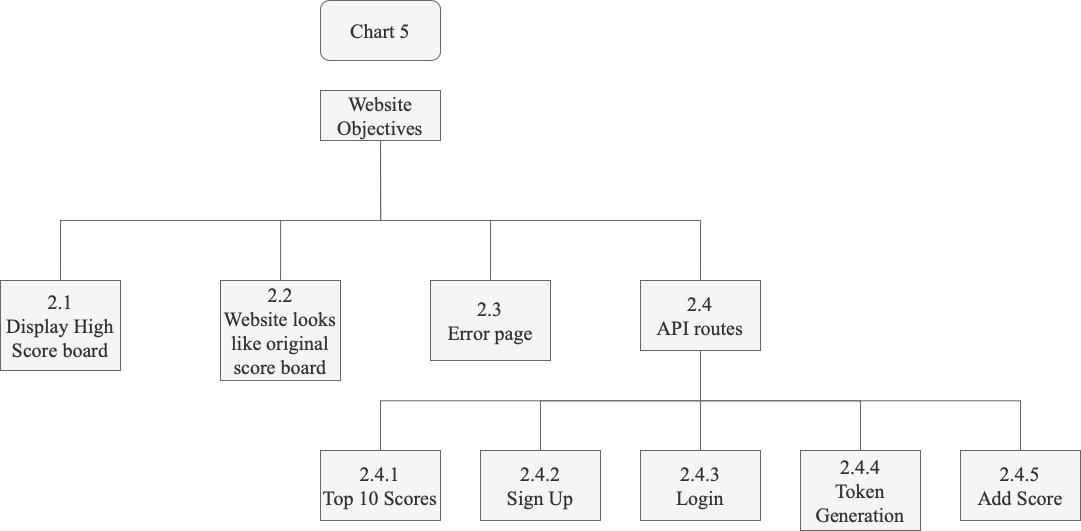
\includegraphics[width=1\linewidth]{Figures/chart5.png}
  \centering
  \caption{Chart detailing website features}
  \label{fig:Chart_5}
\end{figure}

\section{Class Diagrams}
These diagrams define what the actual implementation of classes will be, the first diagram shows that there is a lot of emphasis here on the inheritance and relationships between the classes, its worth noting some of these may extend from default pygame classes, like a surface or sprite, the diagram does show all the classes I have implemented though - along with all of their functions and attributes. 
\begin{figure}[H]
  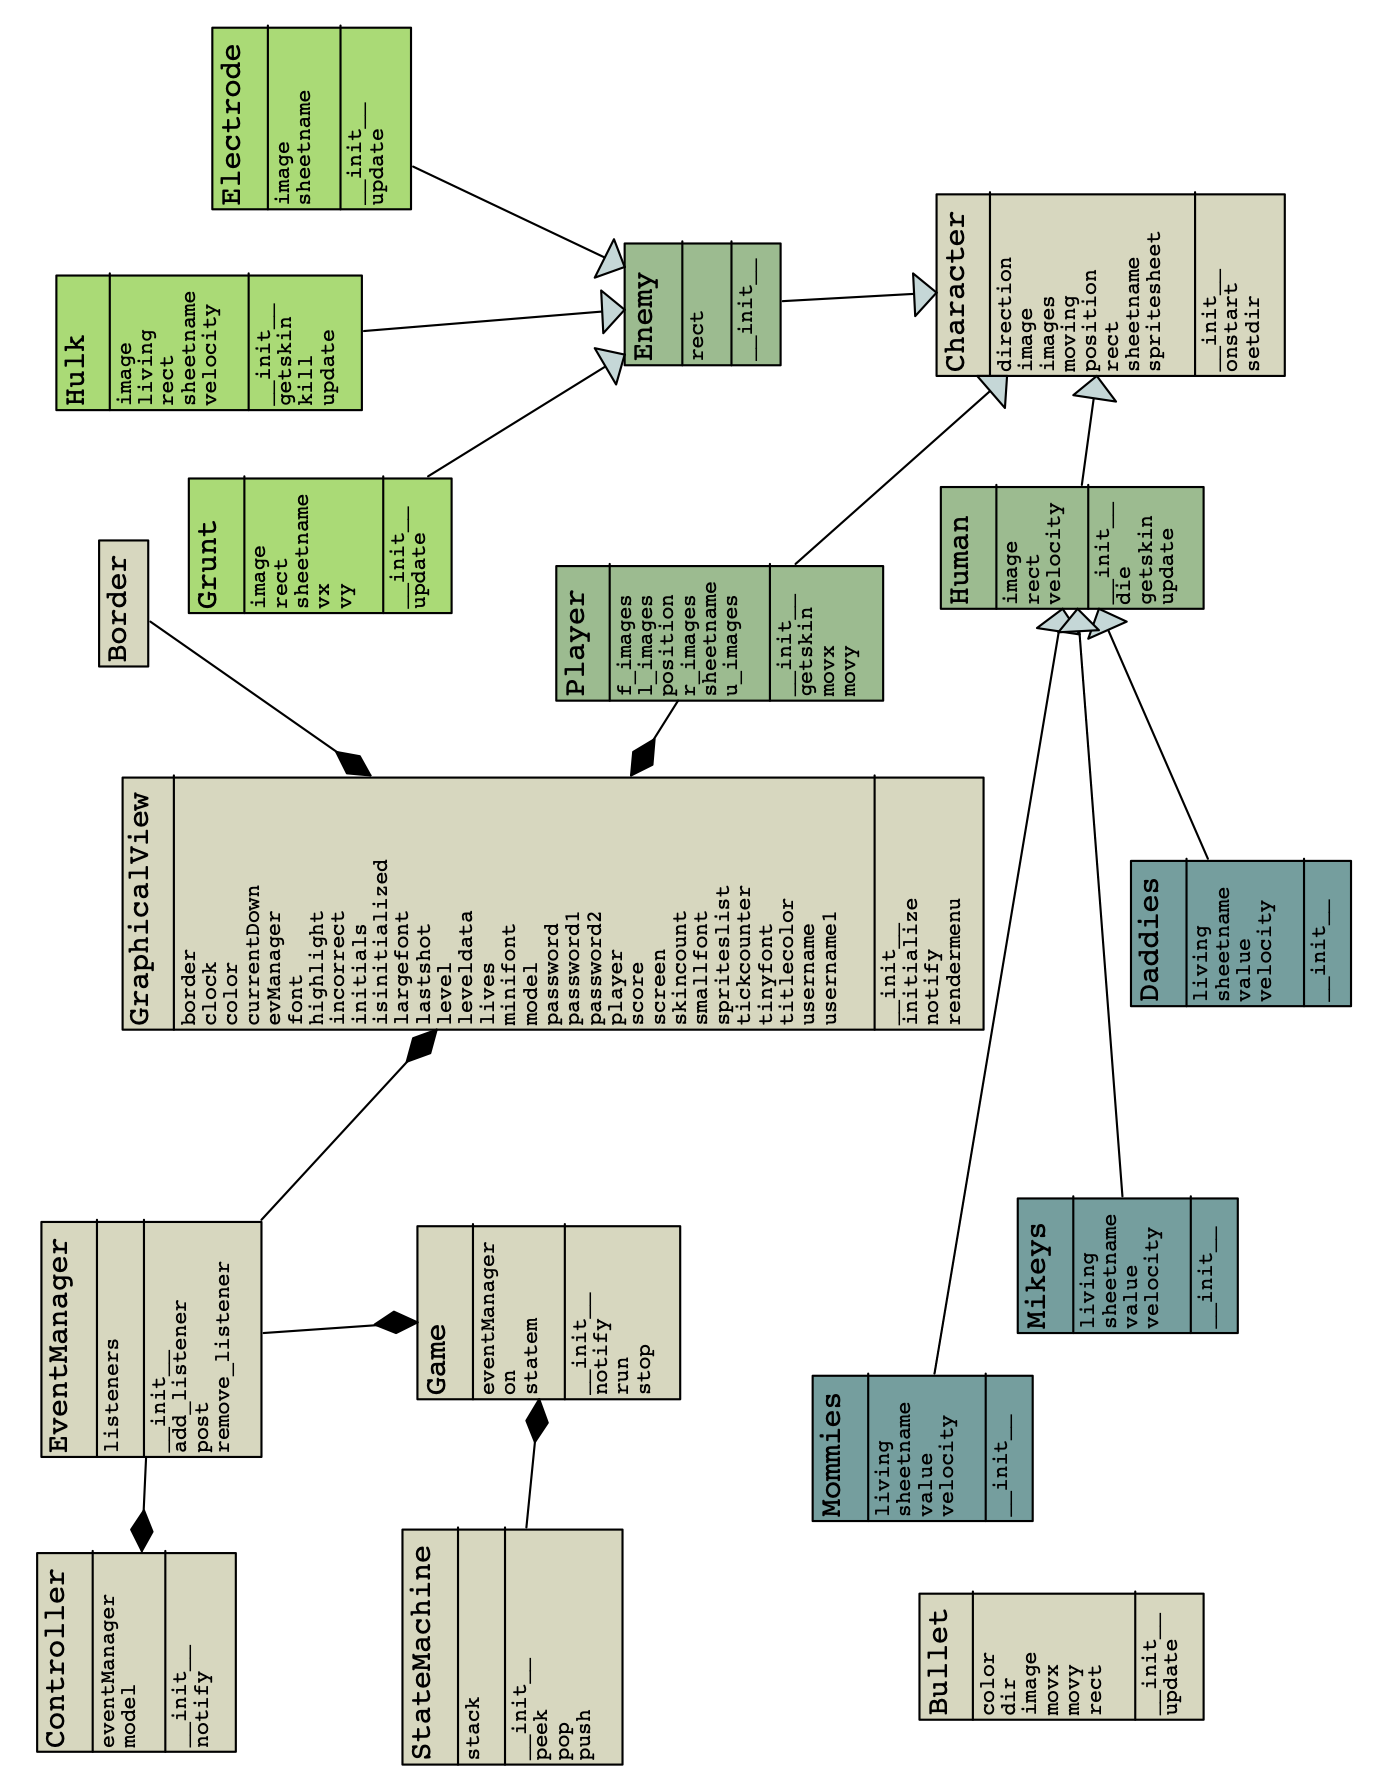
\includegraphics[width=1\linewidth]{Figures/overallclassdiagram.png}
  \centering
  \caption{Class diagrams for the entire system}
  \label{fig:Class_Diagram_MAIN}
\end{figure}

\begin{figure}[H]
  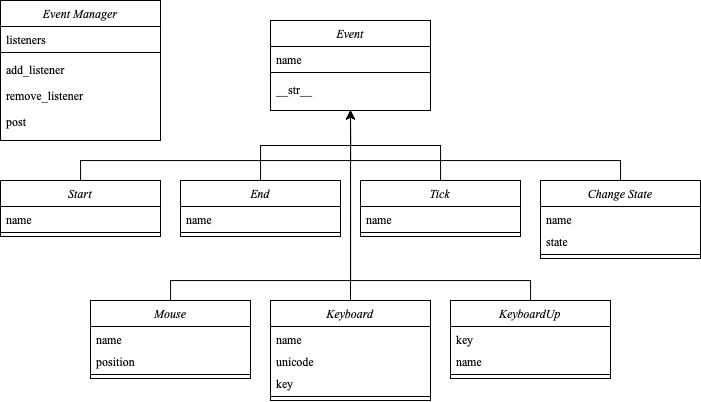
\includegraphics[width=1\linewidth]{Figures/eventclass.png}
  \centering
  \caption{Class diagrams for the events and event manager}
  \label{fig:Class_Diagram_1}
\end{figure}

\begin{figure}[H]
  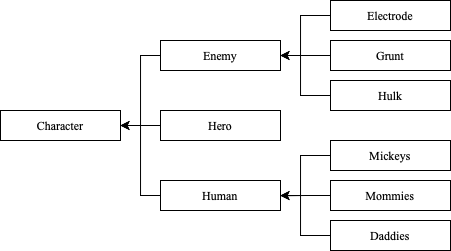
\includegraphics[width=0.6\linewidth]{Figures/charactersDiagram.png}
  \centering
  \caption{Class diagram (with methods and attributes hidden) for characters}
  \label{fig:Class_Diagram_2}
\end{figure}

\begin{figure}[H]
  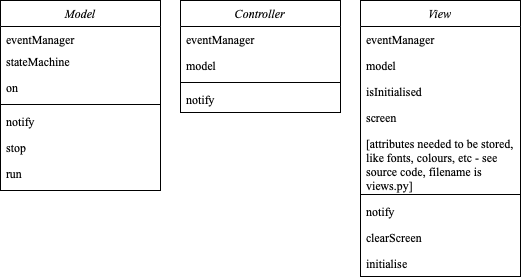
\includegraphics[width=0.8\linewidth]{Figures/MVC0.png}
  \centering
  \caption{Classes required for MVC}
  \label{fig:Class_Diagram_3}
\end{figure}

\section{Key Algorithms}
\subsection{Boids Flocking}
Whilst the maths for this was covered in the  analysis, I will here run through with some pseudo code to show how the moves will be calculated. This pseudo code will be run every time there is a tick emitted (such that the positions are updated every tick - more on ticks in the next section).

\begin{lstlisting}
SUB boids(grunt, gruntlist, playerpos)
    
    # Initialise the variables
    
    x_total, y_total = 0,0
    centre_x ,centre_y = 0,0
    velocity_x, velocity_y = 0,0
    
    # We need this to find all the averages for velocity and positions
    count = len(gruntlist)
    
    # Loop through the grunts on screen
    FOR var_grunt IN gruntlist:

        # Add their positions to the total counts
        x_total += var_grunt.x
        y_total += var_grunt.y
        
        # If they are within 60 pixels of the current grunt - some Pythagoras here
        IF SQRT((var_grunt.x-grunt.x)**2 + (var_grunt.y-grunt.y)**2) < 60 THEN
            # This is the implementation for rule 2 - avoids collisions
            centre_x += centre_x - (var_grunt.x-grunt.x)
            centre_y += centre_y - (var_grunt.y-grunt.y)
            centre_x += (playerpos.x - grunt.x) / 2
            centre_y += (playerpos.y - grunt.y) / 2
        ENDIF
        
        # Add their velocities to the total counts
        velocity_x += var_grunt.velocity_x
        velocity_y += var_grunt.velocity_y
    
    ENDFOR
    
    # Move the grunt closer to the player
    p1 = (playerpos.x-grunt.x) /5
    p2 = (playerpos.y-grunt.y) /5

    # Work out all the averages
    xavg, yavg = x_total/count, y_total/count
    vxavg, vyavg = velocity_x/count, velocity_y/count
    
    # Return (after weighting the rules)
    RETURN (xavg/100)+c1+(vxavg/20)+p1, (yavg/100)+c2+(vyavg/20)+p2
ENDSUB
\end{lstlisting}

\subsection{MVC}
MVC plays a big part in this system and how it works. This is backed by an event and state system too. The class diagrams gave a high level overview of how this works, but no detail into how they interact. This is what will be explained in this section.

Everything is, in reality, centred around the events. These are all controlled by the event manager. The event manager emits messages (or events) to the model, view and controller. These are all received through the 'notify' method on the classes (as each class has this function, the for loop can call the method on all the 'listeners'). The function then decides what it needs to do. Some events may be entirely ignored by the class, whilst others are needed. As such, each event type is its own subclass of the general event. An example of this is the model, which only really relies on the change state and end game events, whilst the view uses all of them.

The states are also needed, the view uses these most of all. The states help it know what generally belongs on screen, whilst the tick counter is what can fine tune that when needed (only certain screens need this, like the menu). So, this flowchart will run through what a basic game might look through.
\begin{figure}[H]
  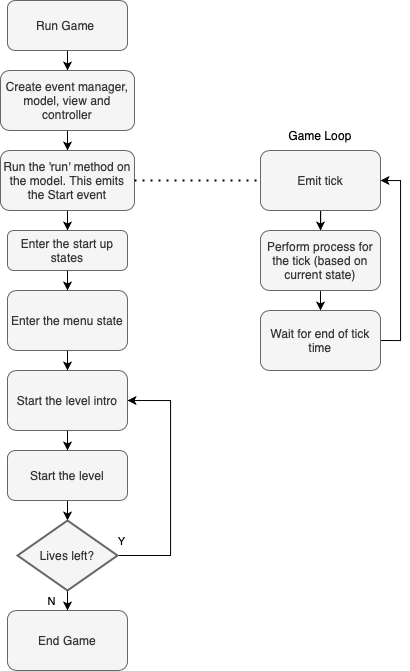
\includegraphics[width=0.7\linewidth]{Figures/flowchart.png}
  \centering
  \caption{Flowchart of how data flows through the system}
  \label{fig:flowchart}
\end{figure}

\subsection{Security}
The project needs security in a few spots. For example, it uses bcrypt, a key derivation algorithm to store passwords. This is much more effective than simply just hashing. It hashes the password, along with salting it, to make it invulnerable to rainbow tables. It then repeats, over and over. This means it takes time to calculate. The idea of a key derivation algorithm over a simple hashing algorithm like SHA is to make computing the result difficult. 

Another aspect where security will be important is in the token generation. If it were possible to guess the token, then a user could authenticate as a different user. As such, I use secrets, specifically the token\_urlsafe, to generate a cryptographically secure, 30 character token. 
\section{Data Structures}
\subsection{Stack}
A stack is a LIFO (last in, first out) data structure. It quite literally acts as a stack of objects. This is what the state machine uses to transition between and store states. This is implemented with a list, objects are both added to and removed from the end, so this is rather simple, but i have included the pseudocode below. 

\begin{lstlisting}
CLASS StateMachine
    stack = []
    
    SUB peek
        TRY
            RETURN stack[-1]
        EXCEPT
            RETURN None
        ENDTRY
    ENDSUB
    
    SUB pop
        TRY
            stack = stack[1:]
            RETURN LEN(stack)
        EXCEPT
            RETURN None
        ENDTRY
    ENDSUB
    
    SUB push(state)
        stack.append(state)
        RETURN state
    ENDSUB
ENDCLASS
\end{lstlisting}
\section{API and Website Design}
The table below shows the routes available on the API, as explained in analysis, this API is used to return the top 10 users, login in, sign up, and validate tokens - forming most of the admin tasks, as well as the website. The website uses a template in flask to show a screen like the original high screen board. The images below show the original and my replica of the high score board. [source for original image \url{http://highscore.com/scores/GameCube/MidwayArcadeTreasures/58417}]

\begin{table}[!ht]
\begin{tabular}{|l|l|l|}
\hline
\rowcolor[HTML]{C0C0C0} 
ROUTE            & METHOD & DESCRIPTION                                                  \\ \hline
/leaderboard     & GET    & Returns JSON of top 10 users (initials + scores) in Database \\ \hline
/user/userid     & GET    & Returns JSON of top score                                    \\ \hline
/username/userid & GET    & Returns ID of given username                                 \\ \hline
/login           & POST   & Logs in a user, sends token, or logs user in with token      \\ \hline
/addscore        & POST   & Adds a score, given score and a token                        \\ \hline
/adduser         & POST   & Adds a user to the database                                  \\ \hline
\end{tabular}
\end{table}


\begin{figure}[H]
  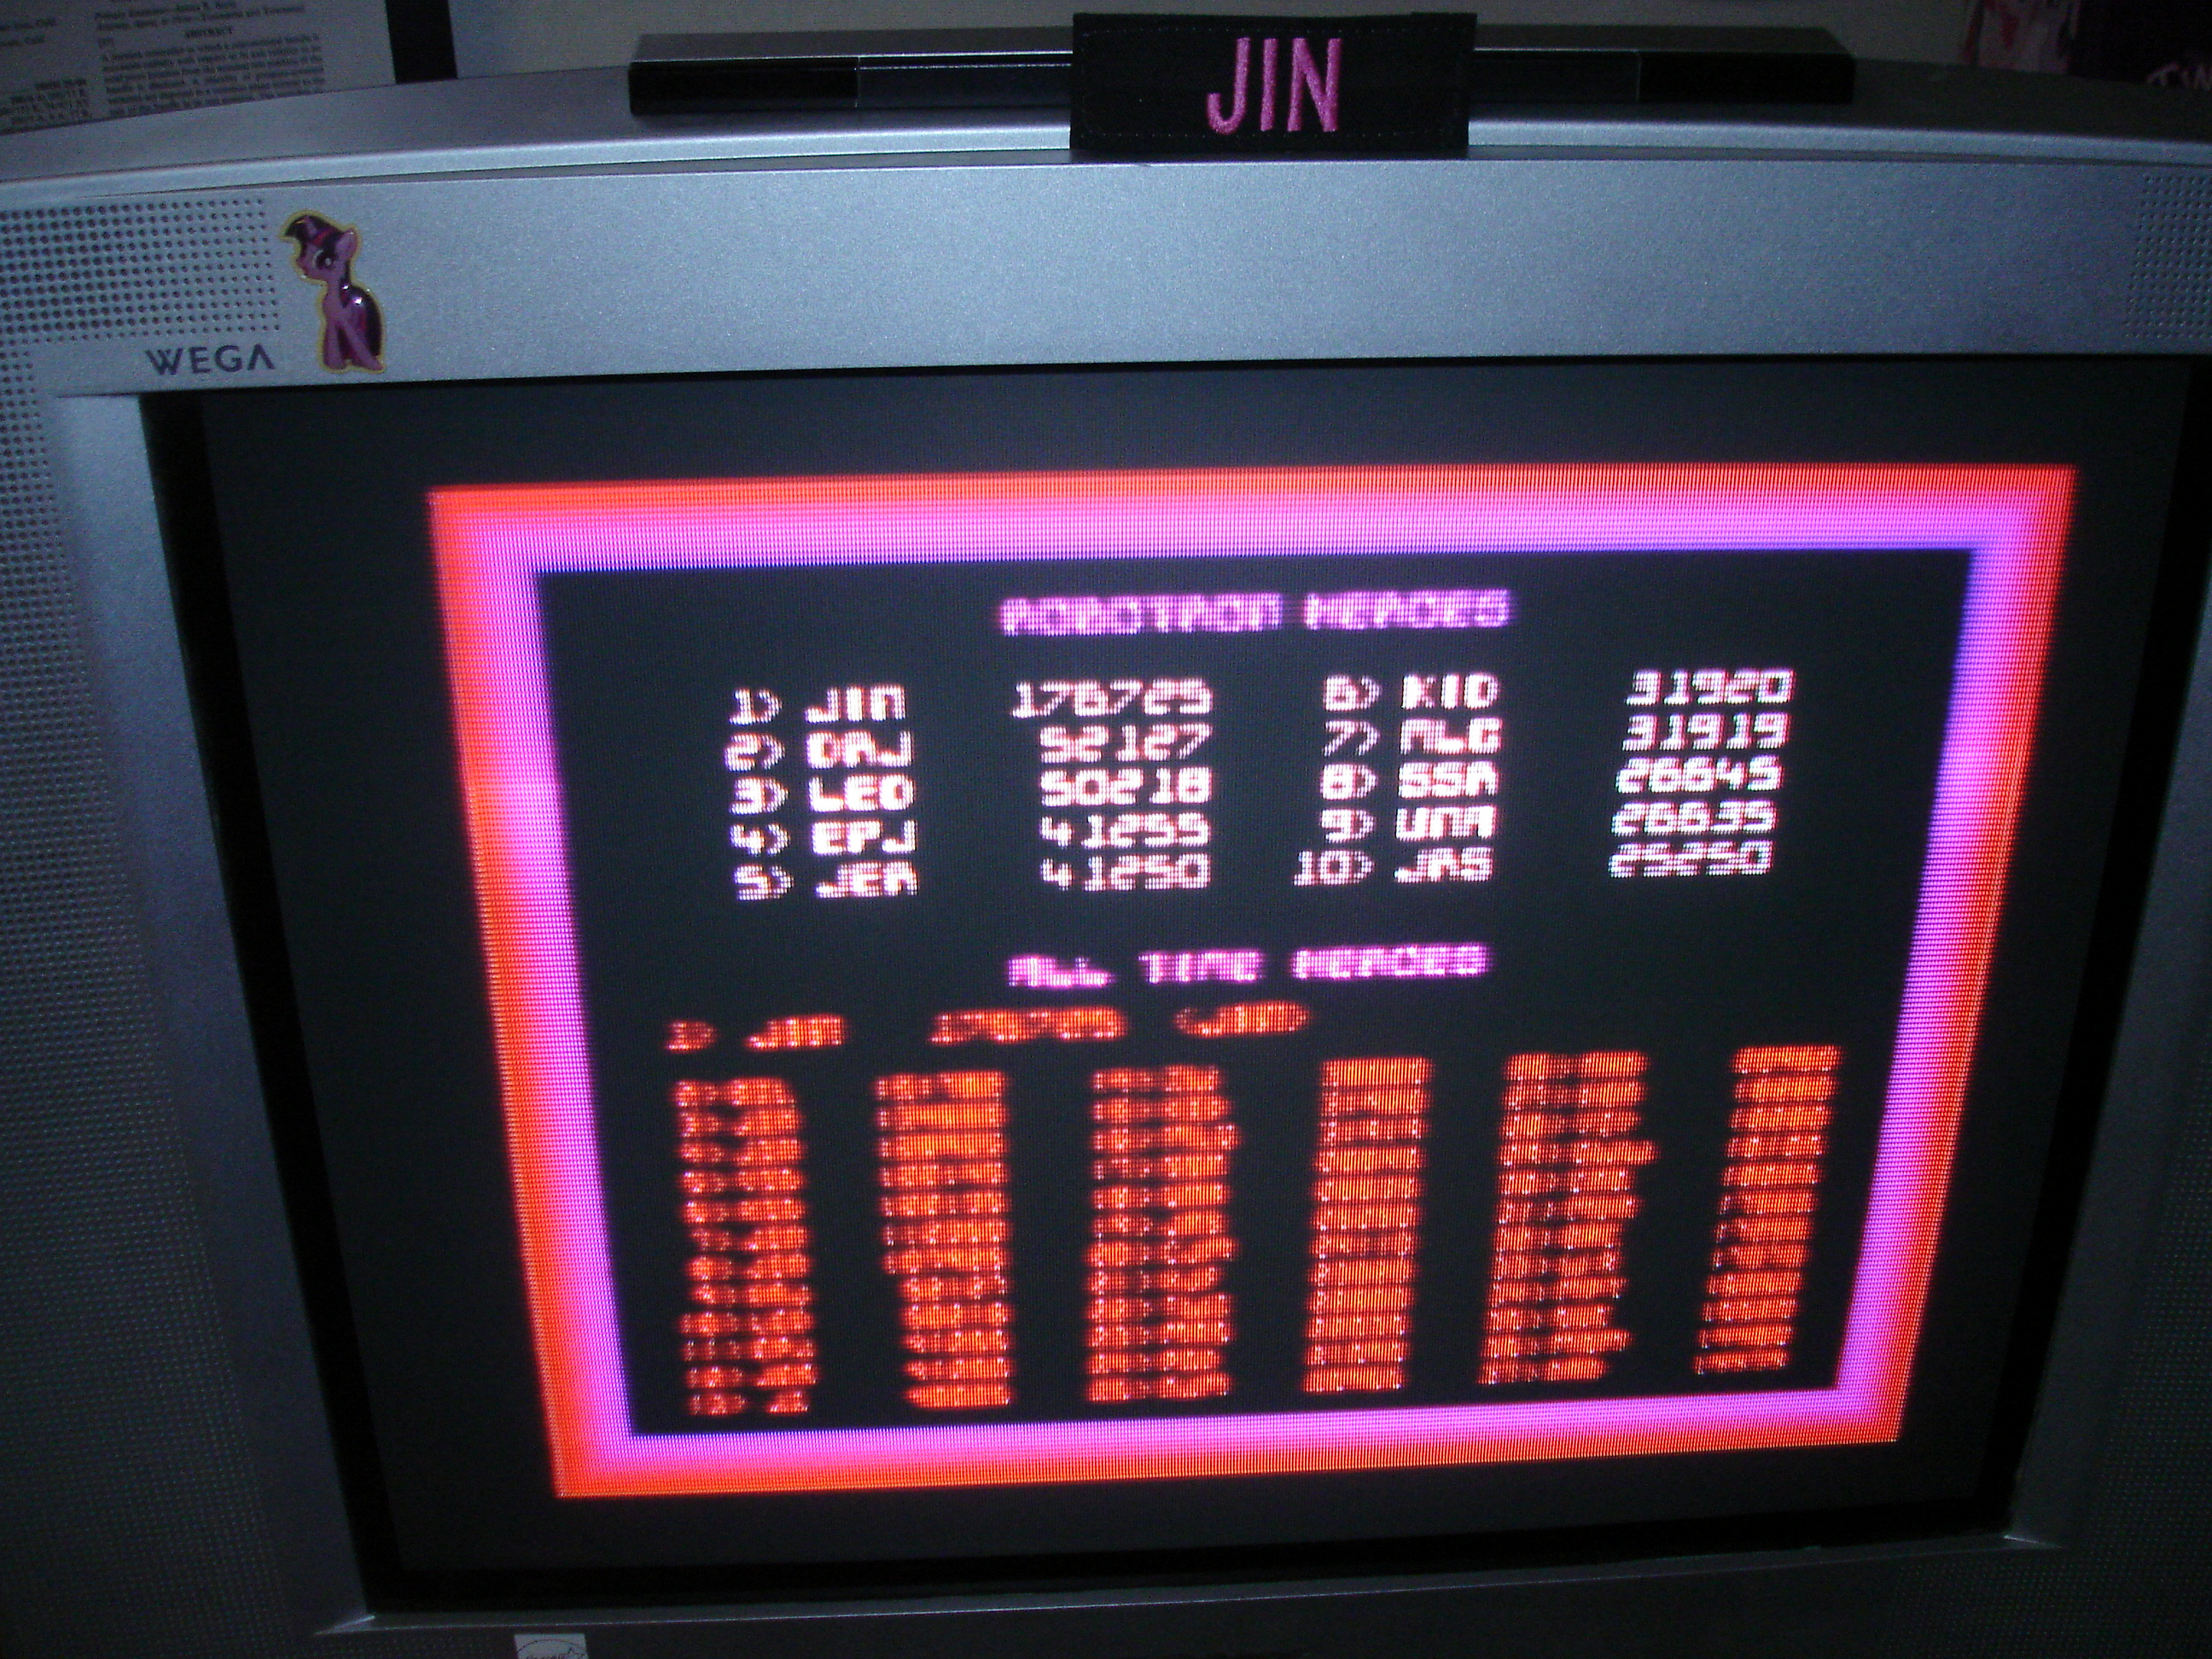
\includegraphics[width=0.8\linewidth]{Figures/web1.jpg}
  \centering
  \caption{Original high score board}
  \label{fig:web1}
\end{figure}


\begin{figure}[H]
  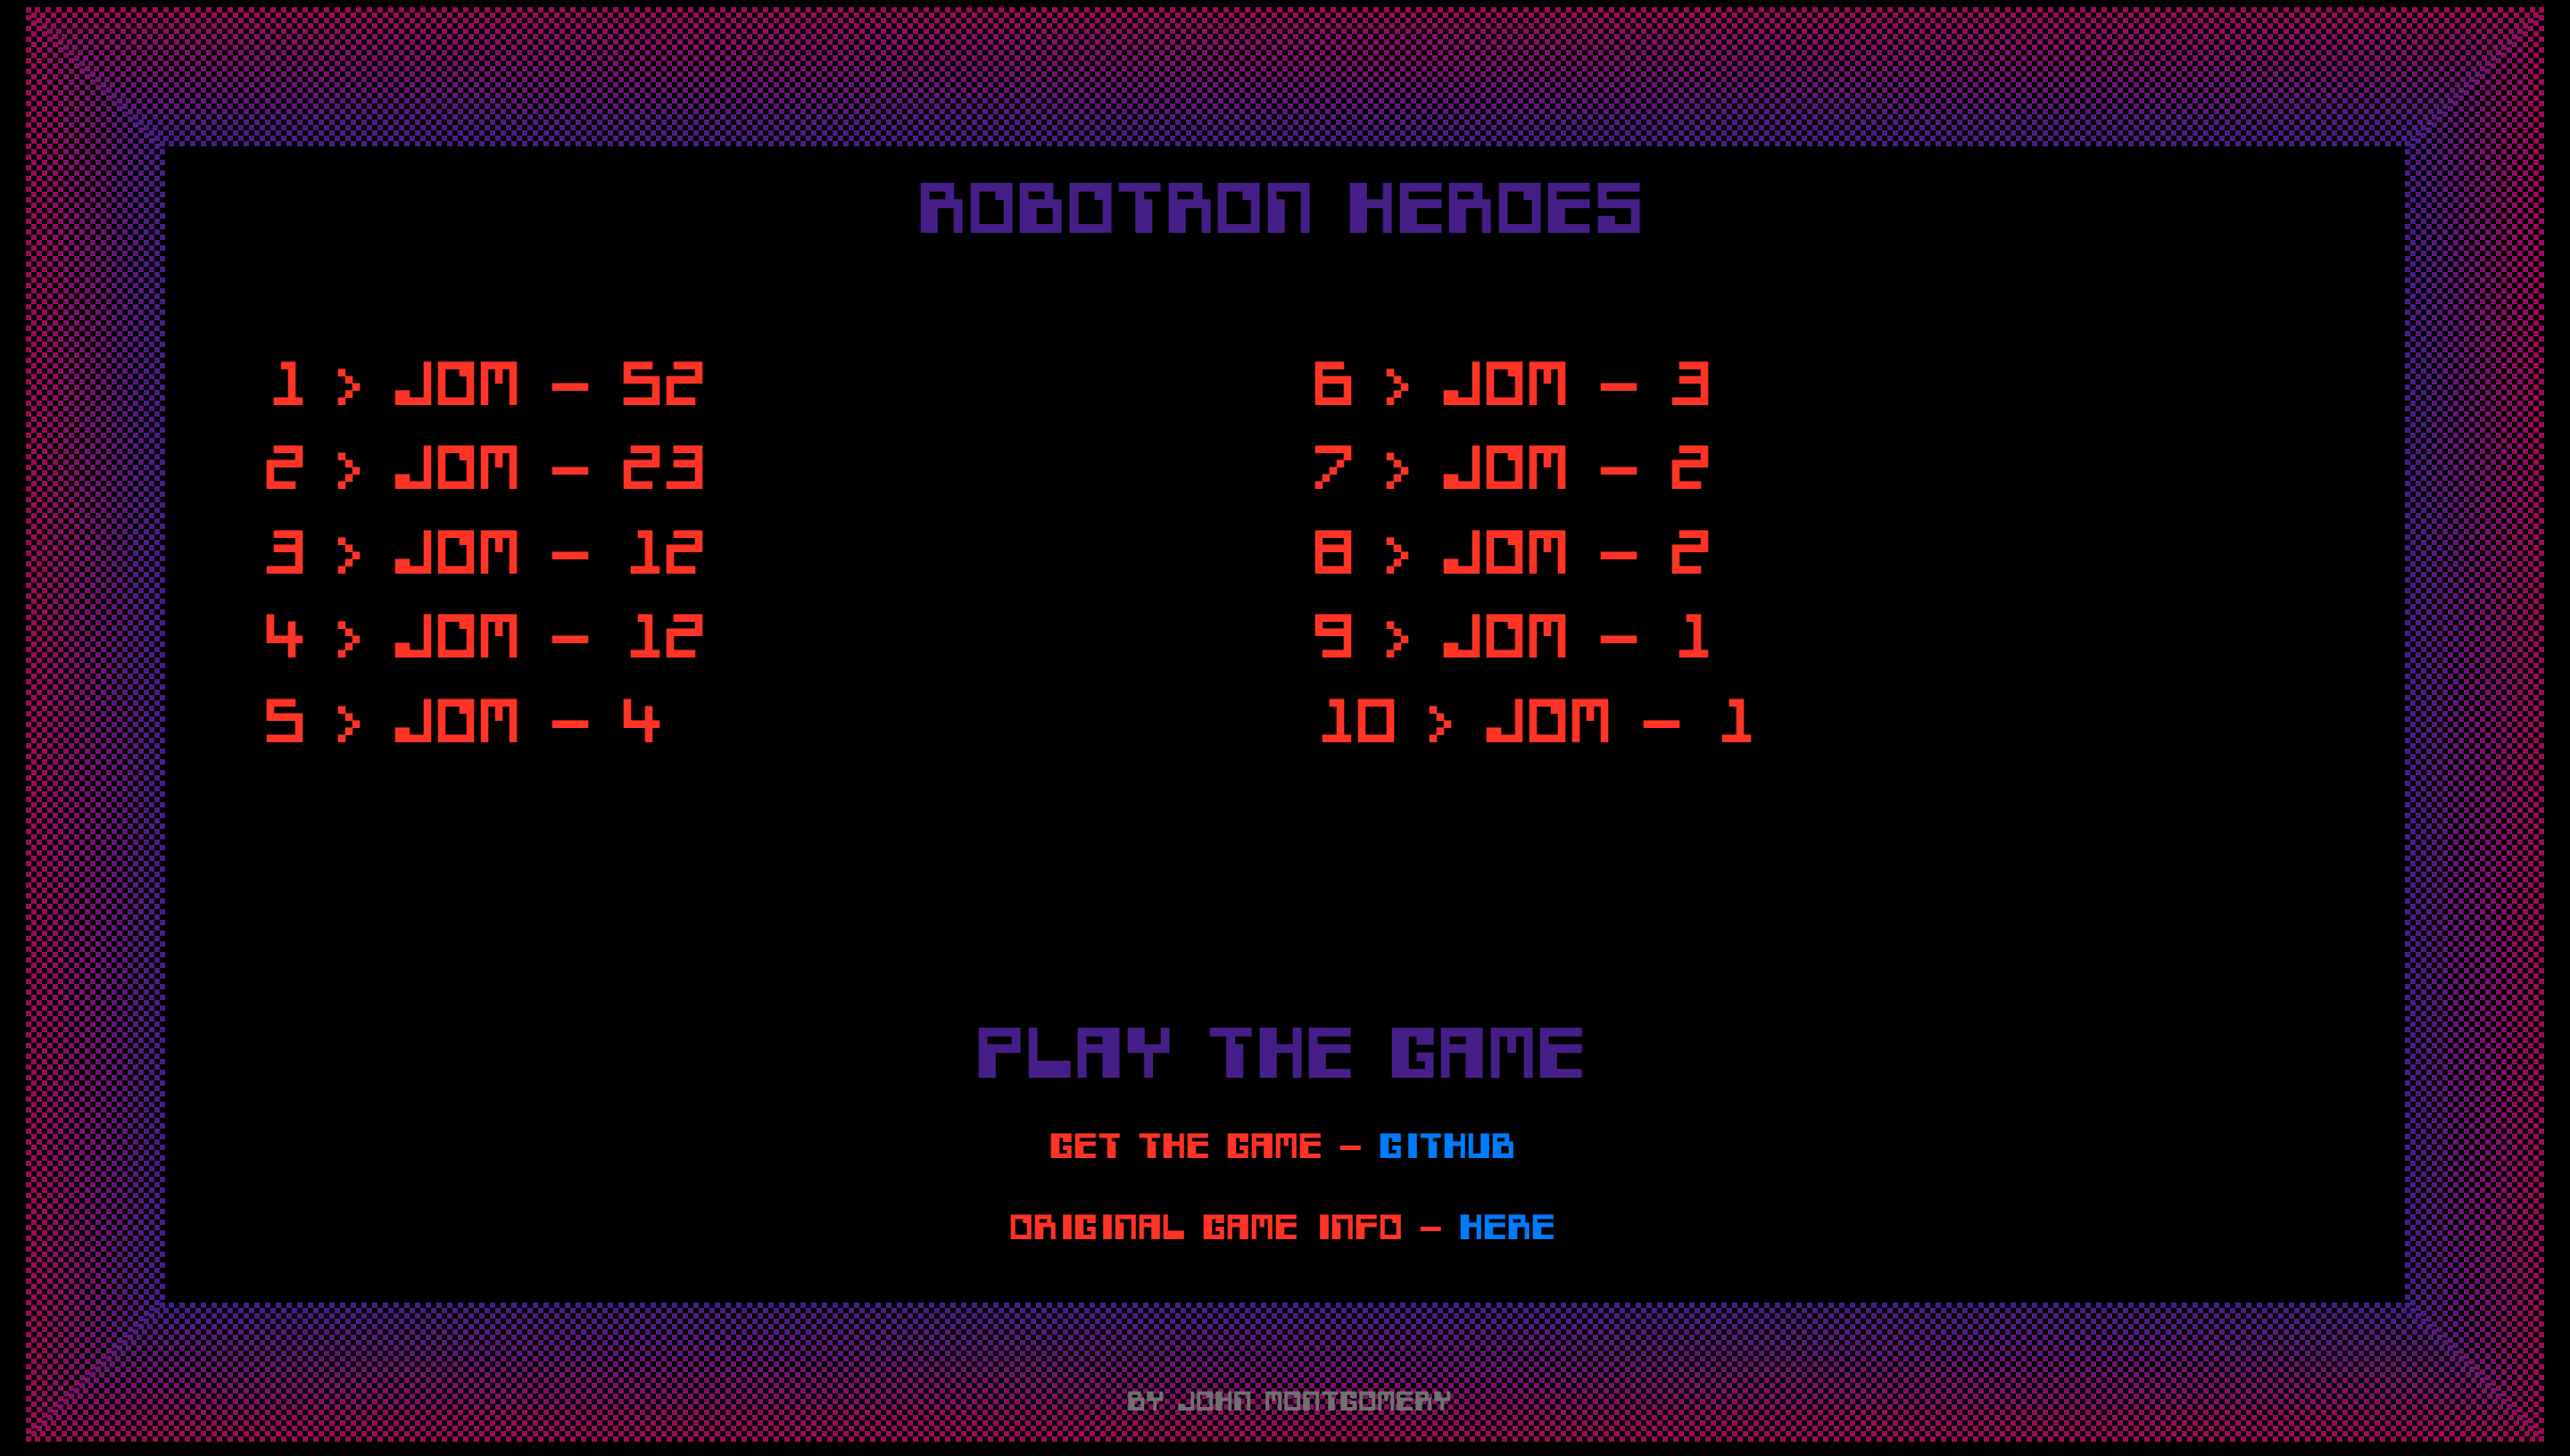
\includegraphics[width=0.8\linewidth]{Figures/web2.png}
  \centering
  \caption{My web implementation of the site}
  \label{fig:web2}
\end{figure}

\section{Database Design}
The database will be needed for the back end of the website, and also is needed in order to make the API work - it stores all the information about the games played, allowing users to login from different clients, and keeps users logged in with tokens, even when they stop running the game. This set up doesn't necessarily need a very complex database set up, it i1s more than proficient with simply having 3 tables, one for main login info, one for scores and one for tokens. The  design puts it into the 3rd normal form to ensure the best time and space efficiency. The SQL statements were tested and written for a sqlite database.

\subsection{Tables (ERD's)}
This diagram shows the database design. It is quite simple, and consists of 2 one to many relationships. One user can have many scores, and one user can have many tokens. This is handled with the foreign key id which allows the tables to be linked, and efficiently get the needed values with join statements.

\begin{figure}[H]
  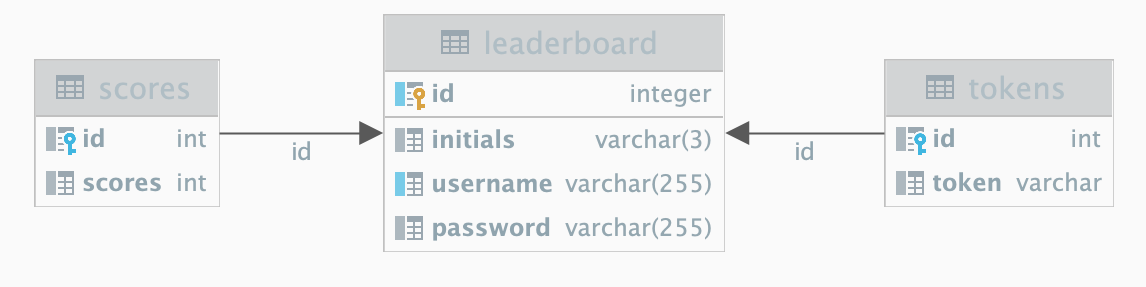
\includegraphics[width=0.8\linewidth]{Figures/leaderboard.png}
  \centering
  \caption{ERD showing the database design}
  \label{fig:ERD}
\end{figure}

\subsection{Queries}
This section will detail all the queries used in the code, in order of how they are found in the file, it just so happens this is also essentially in order of the complexity. The first query is run every time the flask server is run. By using 'IF NOT EXISTS' i am able to ensure that the table will be there when needed, but also that restarting the server will not remove any data which is stored in the file. 

\begin{figure}[H]
    \begin{lstlisting}[language=SQL, style=mystyle1]
CREATE TABLE IF NOT EXISTS leaderboard (
    id INTEGER UNIQUE PRIMARY KEY AUTOINCREMENT,
    initials VARCHAR(3),
    username VARCHAR(255) UNIQUE,
    password VARCHAR(255)
);
CREATE TABLE IF NOT EXISTS scores(
    id INT references leaderboard,
    scores INT
);
CREATE TABLE IF NOT EXISTS tokens (
    id INT references leaderboard,
    token VARCHAR
);
    \end{lstlisting}
      \centering
      \caption{Create table queries}
      \label{fig:SQL1}
\end{figure}

This select is used to return the top 10 scorers in the database, deconstructing it, we can see we are selecting the initials and scores, from the leader board table, joined to the scores table, on the id's. Next we want to order by the scores to ensure we get the top 10, and then only select 10 items
\begin{figure}[H]
    \begin{lstlisting}[language=SQL, style=mystyle1]
SELECT leaderboard.initials, scores
FROM leaderboard
LEFT JOIN scores
ON leaderboard.id = scores.id
ORDER BY scores DESC
LIMIT 10;
    \end{lstlisting}
      \centering
      \caption{Query to get the top 10 scorers and the initals linked to them}
      \label{fig:SQL2}
\end{figure}


\begin{figure}[H]
    \begin{lstlisting}[language=SQL, style=mystyle1]
SELECT leaderboard.id
FROM leaderboard
WHERE leaderboard.username = {username}
LIMIT 1;
    \end{lstlisting}
      \centering
      \caption{Query to get the id of a user given their unique username}
      \label{fig:SQL3}
\end{figure}

\begin{figure}[H]
    \begin{lstlisting}[language=SQL, style=mystyle1]
SELECT password
FROM leaderboard
WHERE leaderboard.id = {userid}
LIMIT 1;
    \end{lstlisting}
      \centering
      \caption{Query to get the hashed password info for a given id}
      \label{fig:SQL4}
\end{figure}

\begin{figure}[H]
    \begin{lstlisting}[language=SQL, style=mystyle1]
SELECT token
FROM tokens
WHERE id = {userid}
LIMIT 1;
    \end{lstlisting}
      \centering
      \caption{Query to get the token for a given id}
      \label{fig:SQL5}
\end{figure}

\begin{figure}[H]
    \begin{lstlisting}[language=SQL, style=mystyle1]
INSERT INTO tokens (id, token)
VALUES ('{userid}','{token}');
    \end{lstlisting}
      \centering
      \caption{Query to insert the token values}
      \label{fig:SQL6}
\end{figure}

\begin{figure}[H]
    \begin{lstlisting}[language=SQL, style=mystyle1]
INSERT INTO scores (id, scores)
VALUES ({userid},{score});
    \end{lstlisting}
      \centering
      \caption{Query to insert a new score}
      \label{fig:SQL7}
\end{figure}

\begin{figure}[H]
    \begin{lstlisting}[language=SQL, style=mystyle1]
INSERT INTO leaderboard (initials, username, password)
VALUES ('{initials}','{username}','{tostore}');
    \end{lstlisting}
      \centering
      \caption{Query to insert a new score}
      \label{fig:SQL8}
\end{figure}



\section{HCI}
Human Computer Interaction designs are going to be taken from the pygame itself, as this is how my program was built. I will also show some screens from the original game, all of which are taken from the links which can be found in the analysis section. The font is found at \url{https://fontstruct.com/fontstructions/show/474939/robotron_2084} and is under a creative commons license.

\newpage
This screen we can see a bunch of random coloured squares, this is designed to look just like what startup did on the original arcade game of this. It has no real features to mention
\begin{figure}[H]
  \includegraphics[width=1\linewidth]{Figures/random.png}
  \centering
  \caption{Random screen shown}
  \label{fig:HCI1}
\end{figure}
\newpage
This testing screen (whilst probably useful for the original) is not functional, but gives a but more of the sense of the game. 
\begin{figure}[H]
  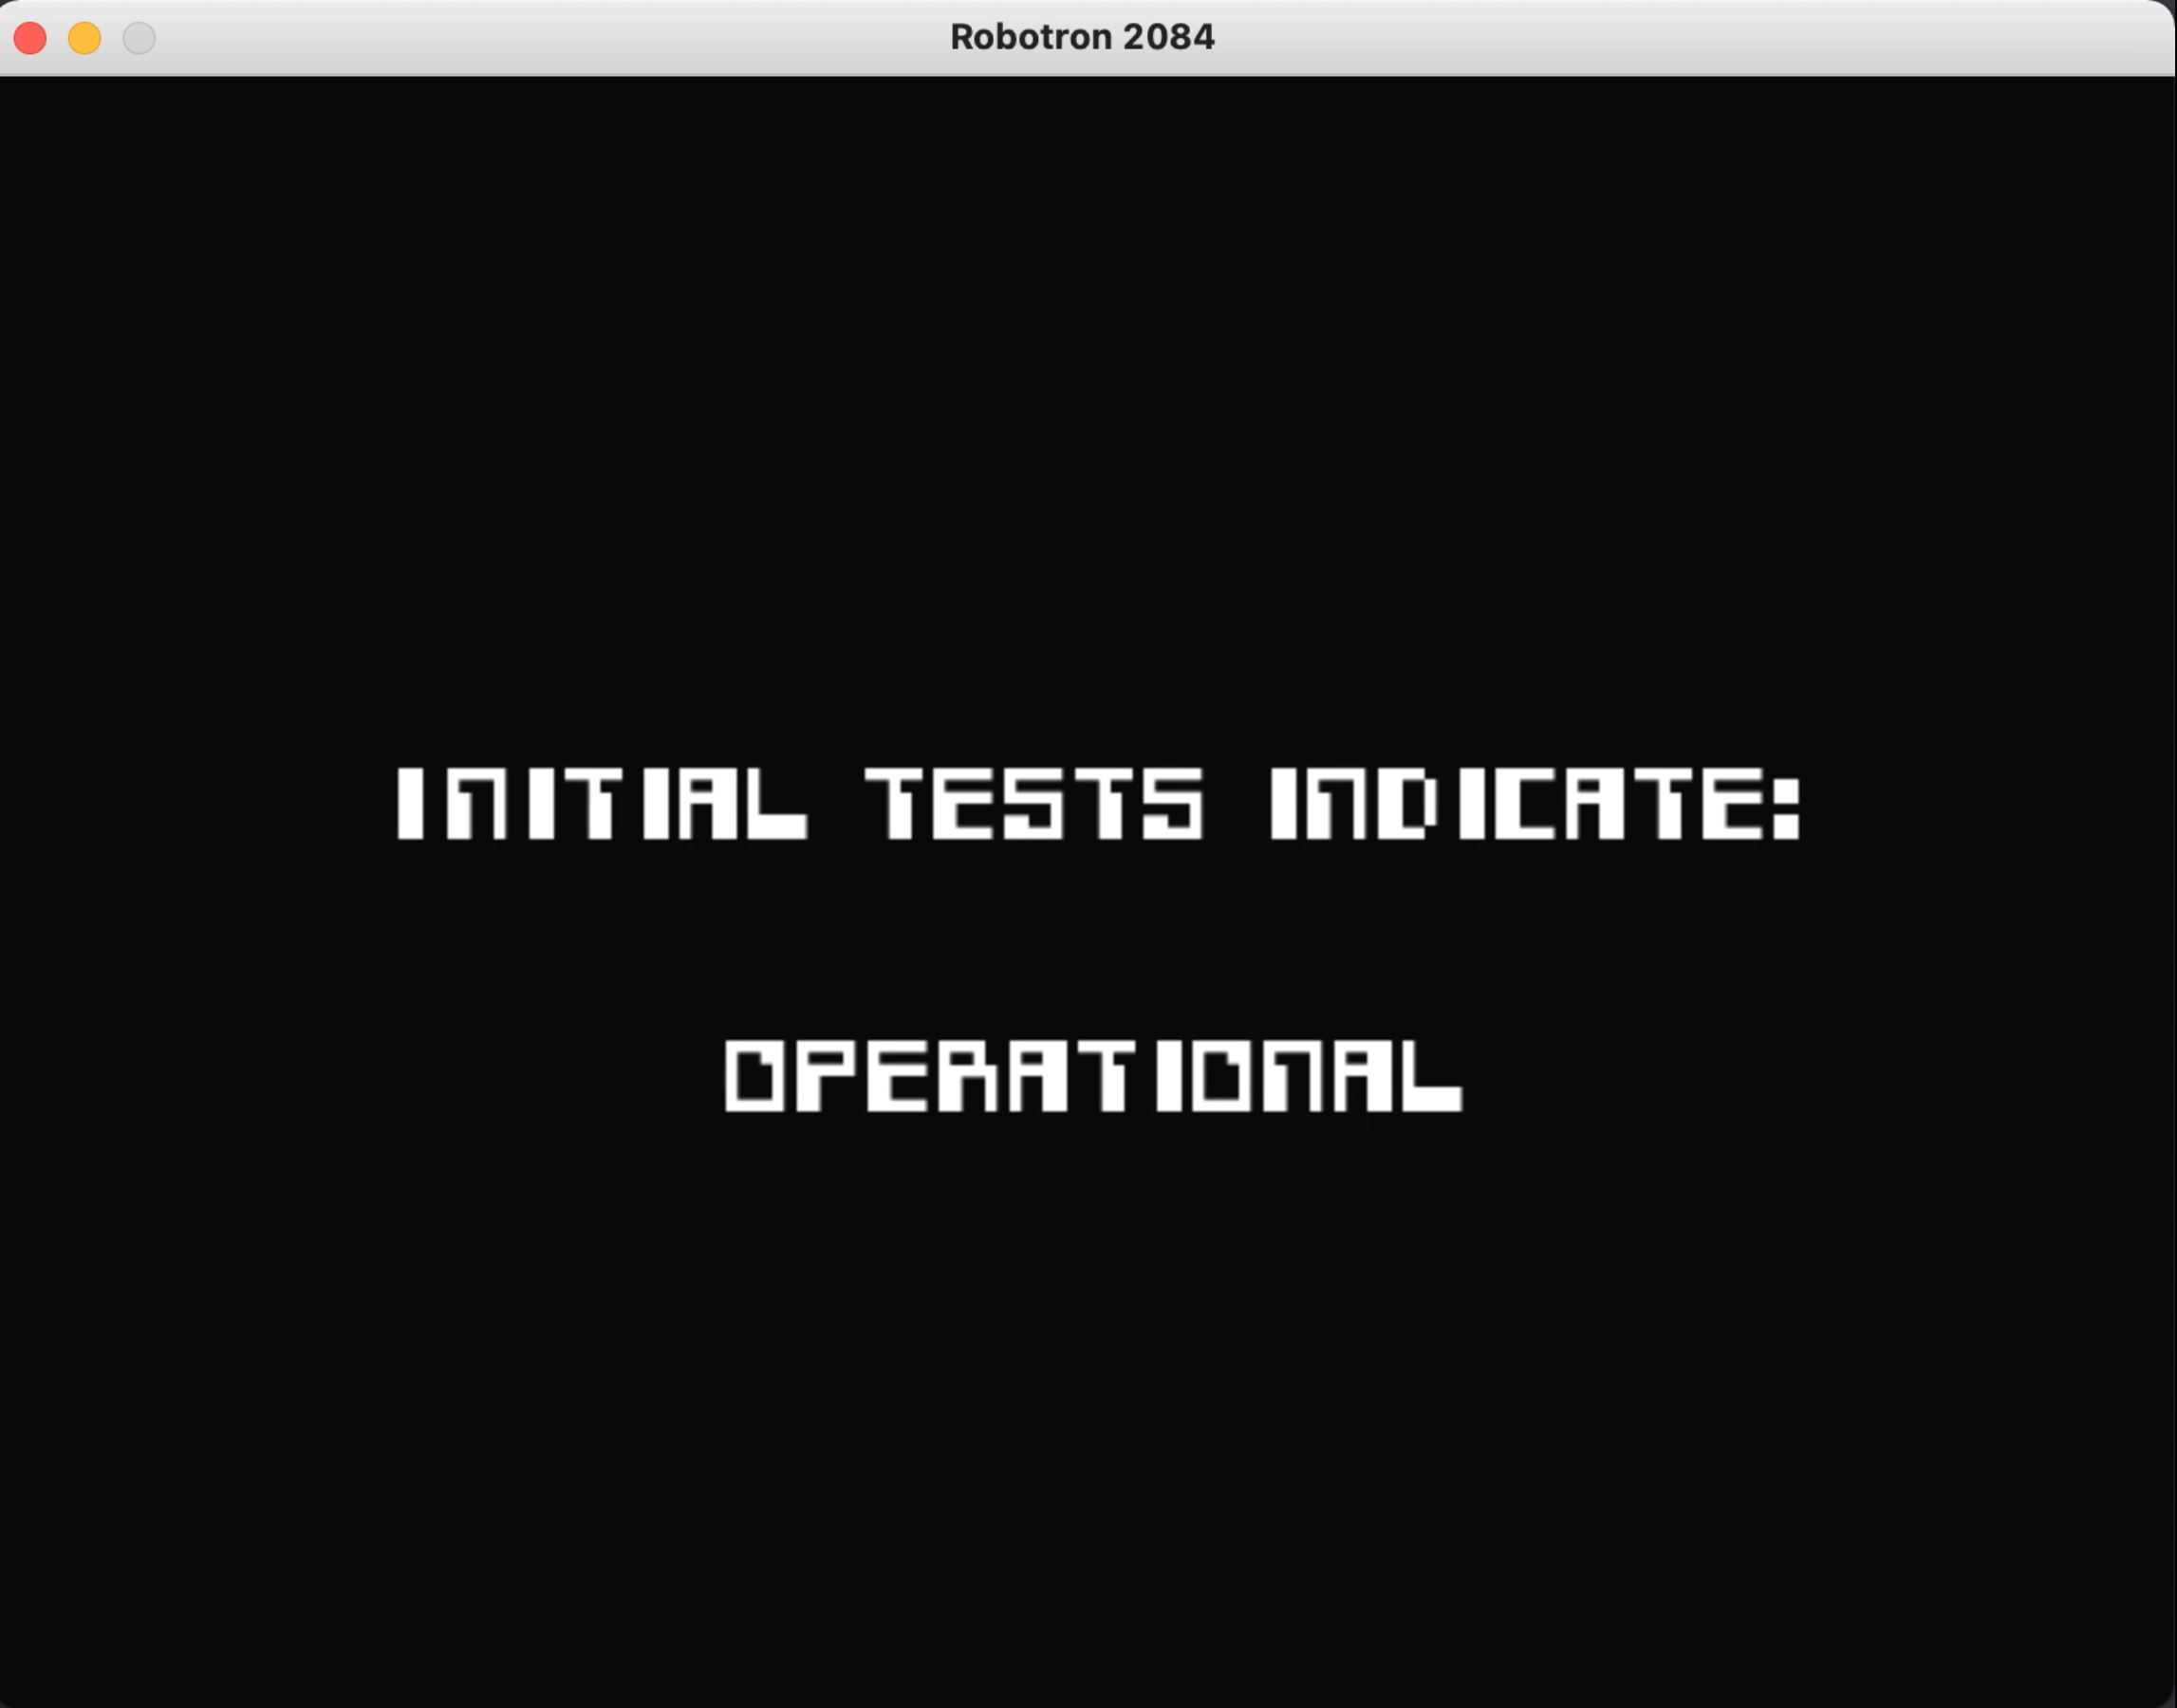
\includegraphics[width=1\linewidth]{Figures/tests.png}
  \centering
  \caption{Testing screen}
  \label{fig:HCI2}
\end{figure}

\newpage
This is the first part where users can actually interact, and it is a first into into the very fast pace of the game, with all the flashing colours and other rapidly changing features. This is where users can log in, play and get info like the leaderboard link.
\begin{figure}[H]
  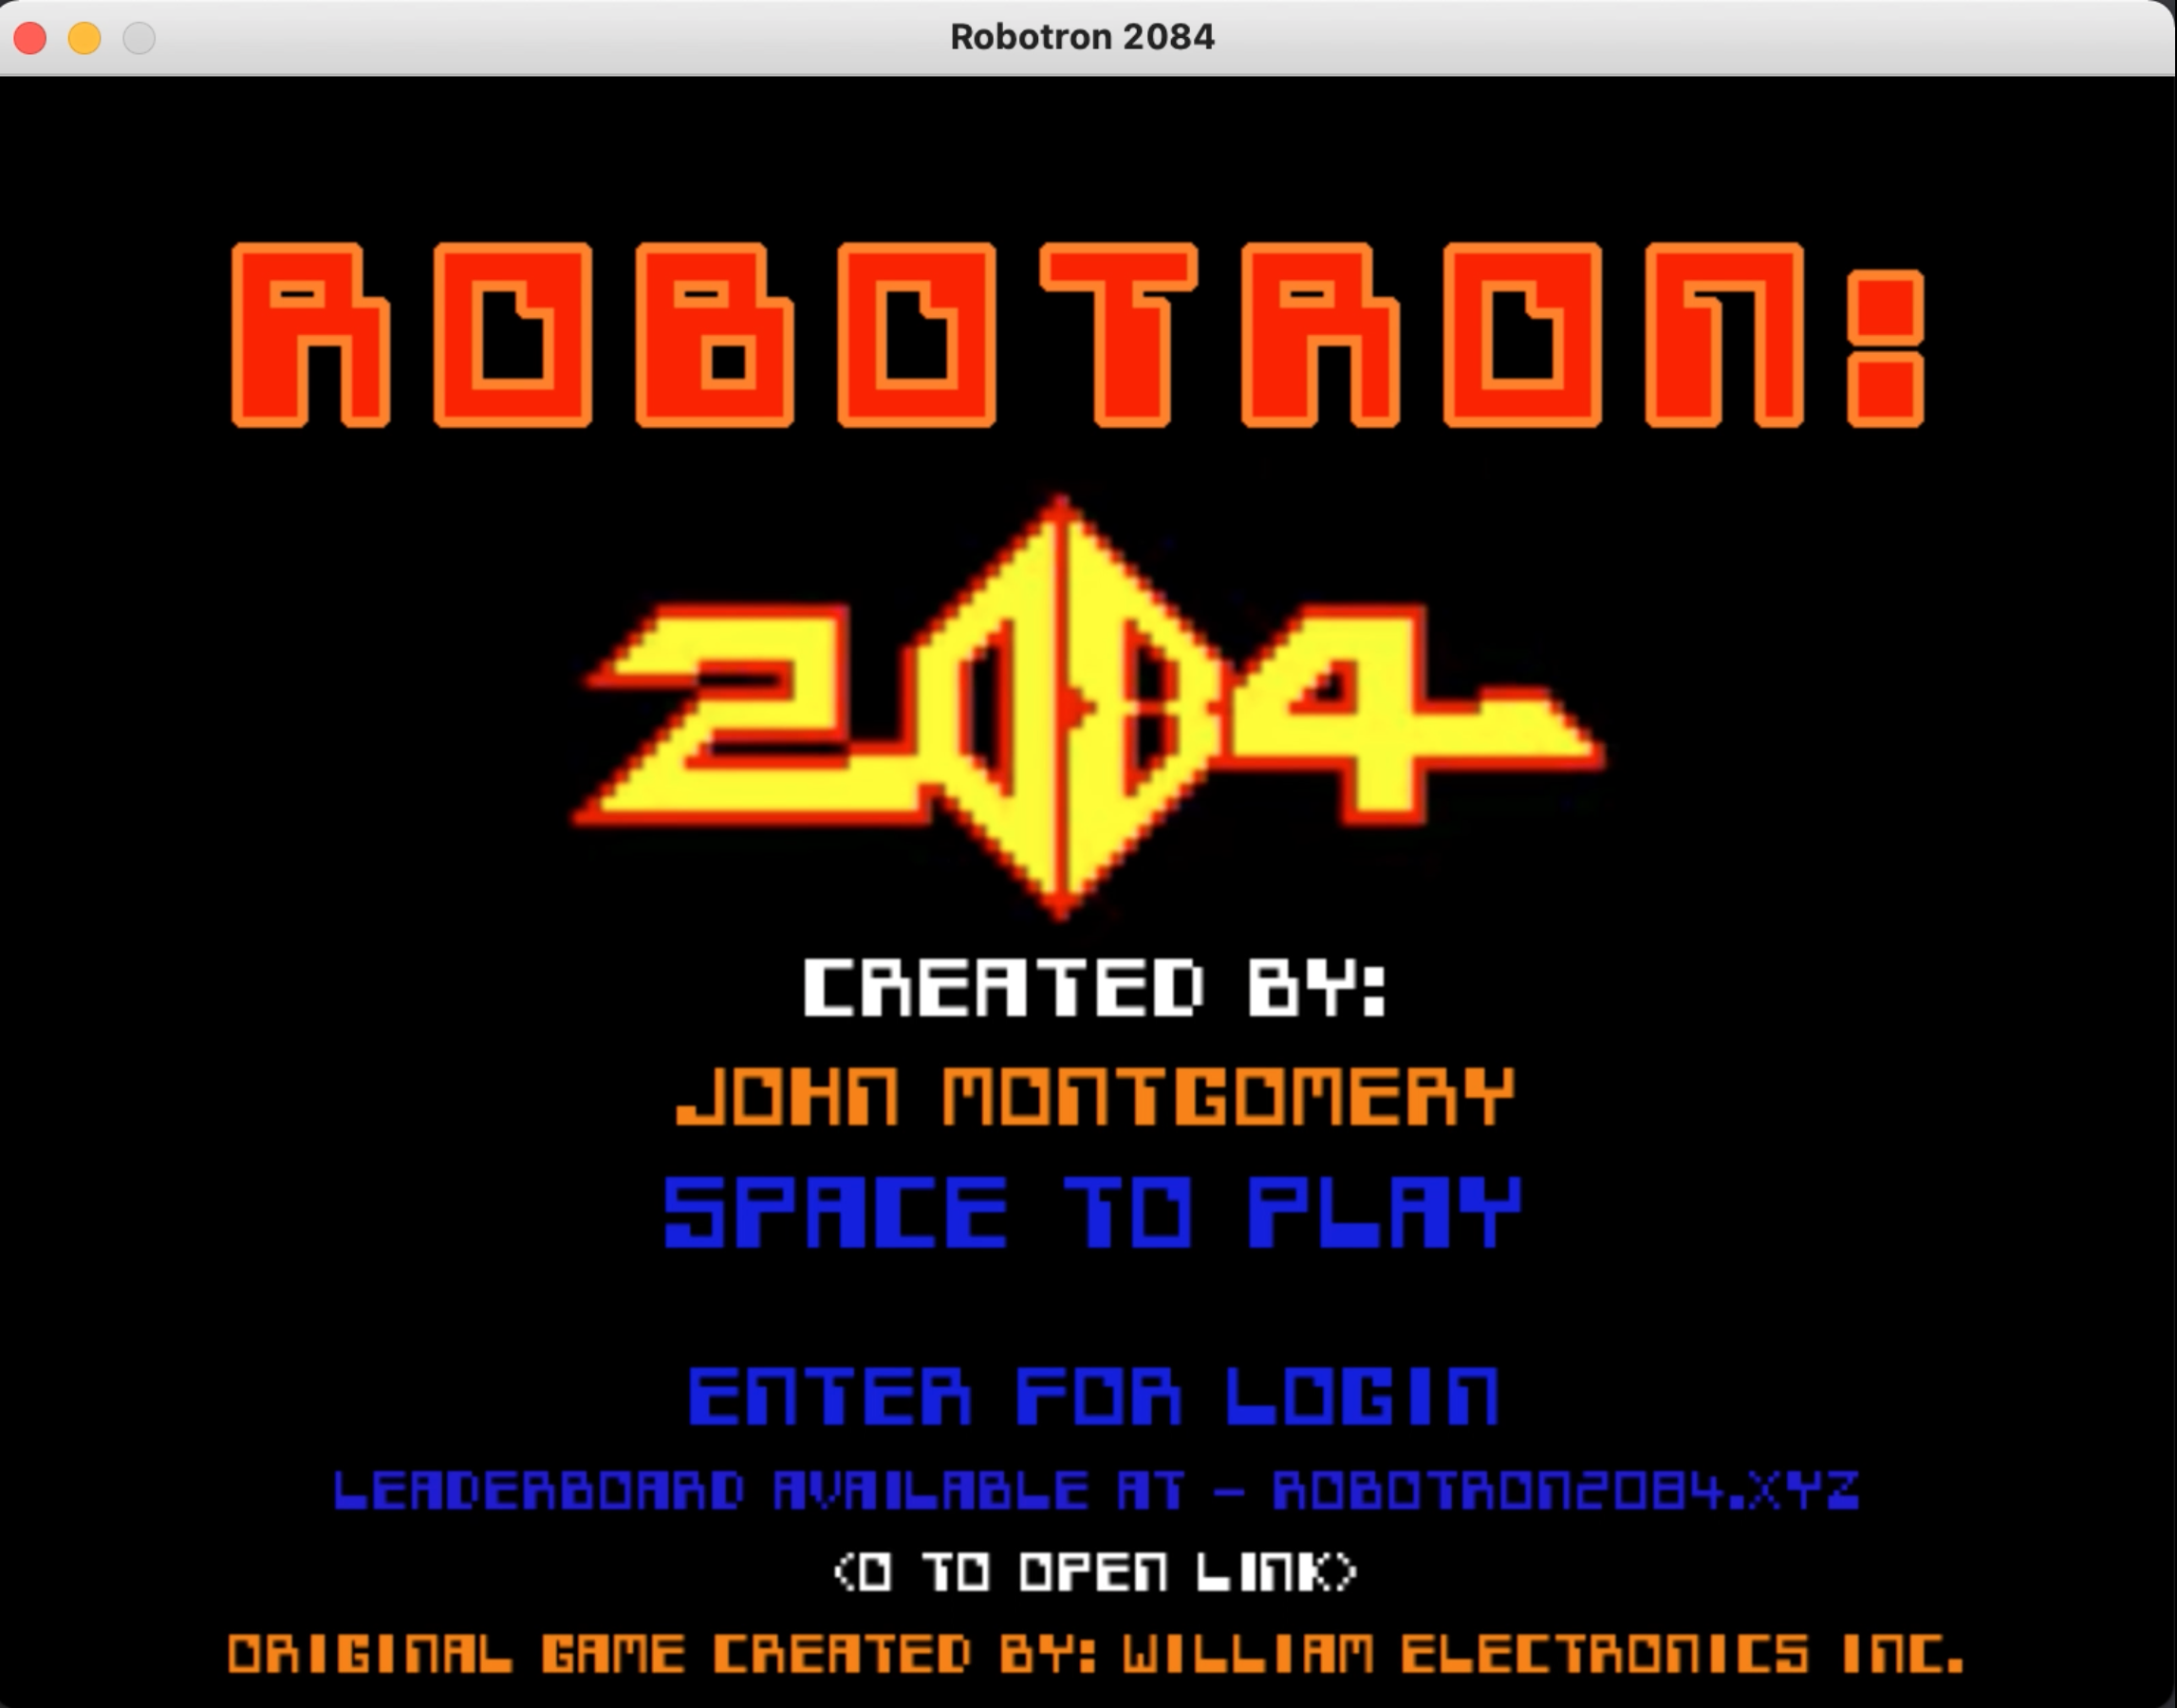
\includegraphics[width=1\linewidth]{Figures/menu.png}
  \centering
  \caption{Menu}
  \label{fig:HCI3}
\end{figure}
\newpage
This page is where the user logs in, it needs to be fairly basic, and it doesnt have all the flashing colours and brightness. The boxes get 'highlighted' when clicked, and there is a back button in the top left. The boxes also get bordered in red when the inputs are invalid, whether from an incorrect password or from other issues, like too short passwords.
\begin{figure}[H]
  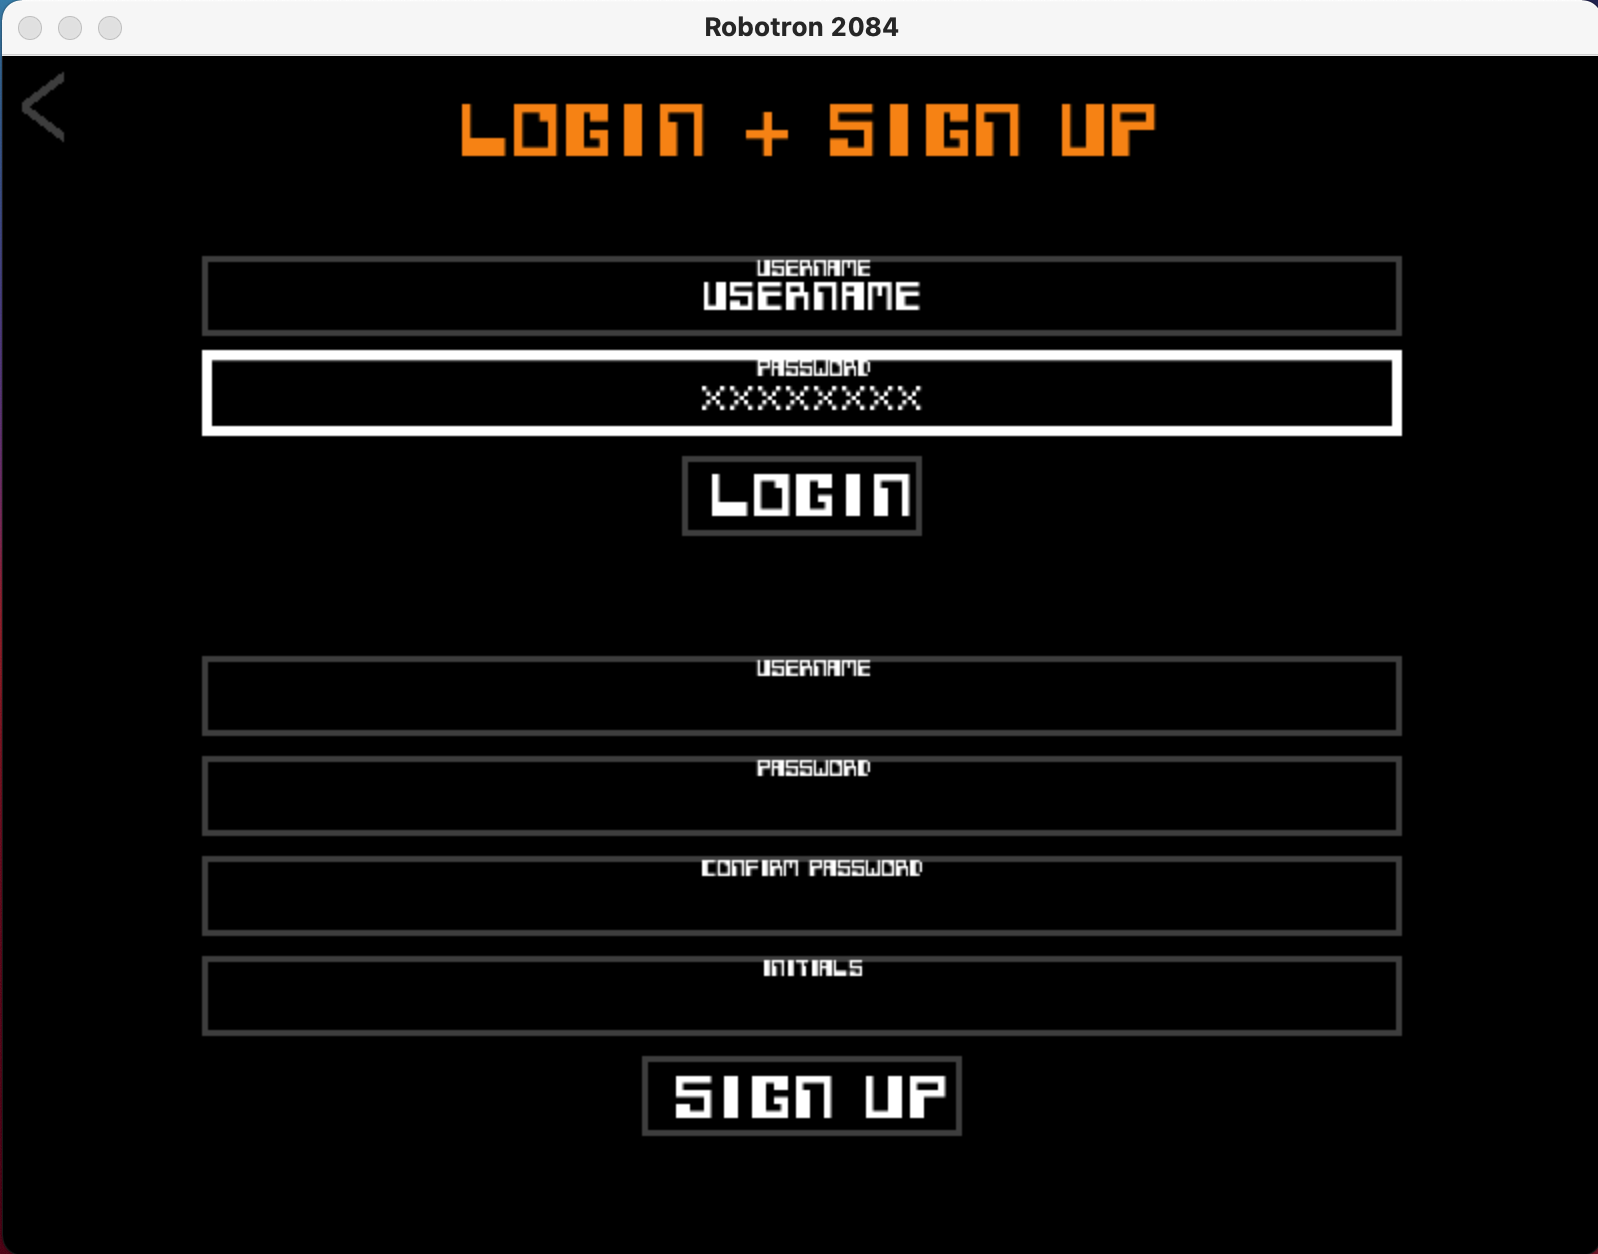
\includegraphics[width=1\linewidth]{Figures/login.png}
  \centering
  \caption{Login and sign up page}
  \label{fig:HCI4}
\end{figure}
\newpage
Theres not much variation from the original for this. Its very quick, and looks a lot like the basic game, bullets are random colours, and the border flashes, along with the life counter.
\begin{figure}[H]
  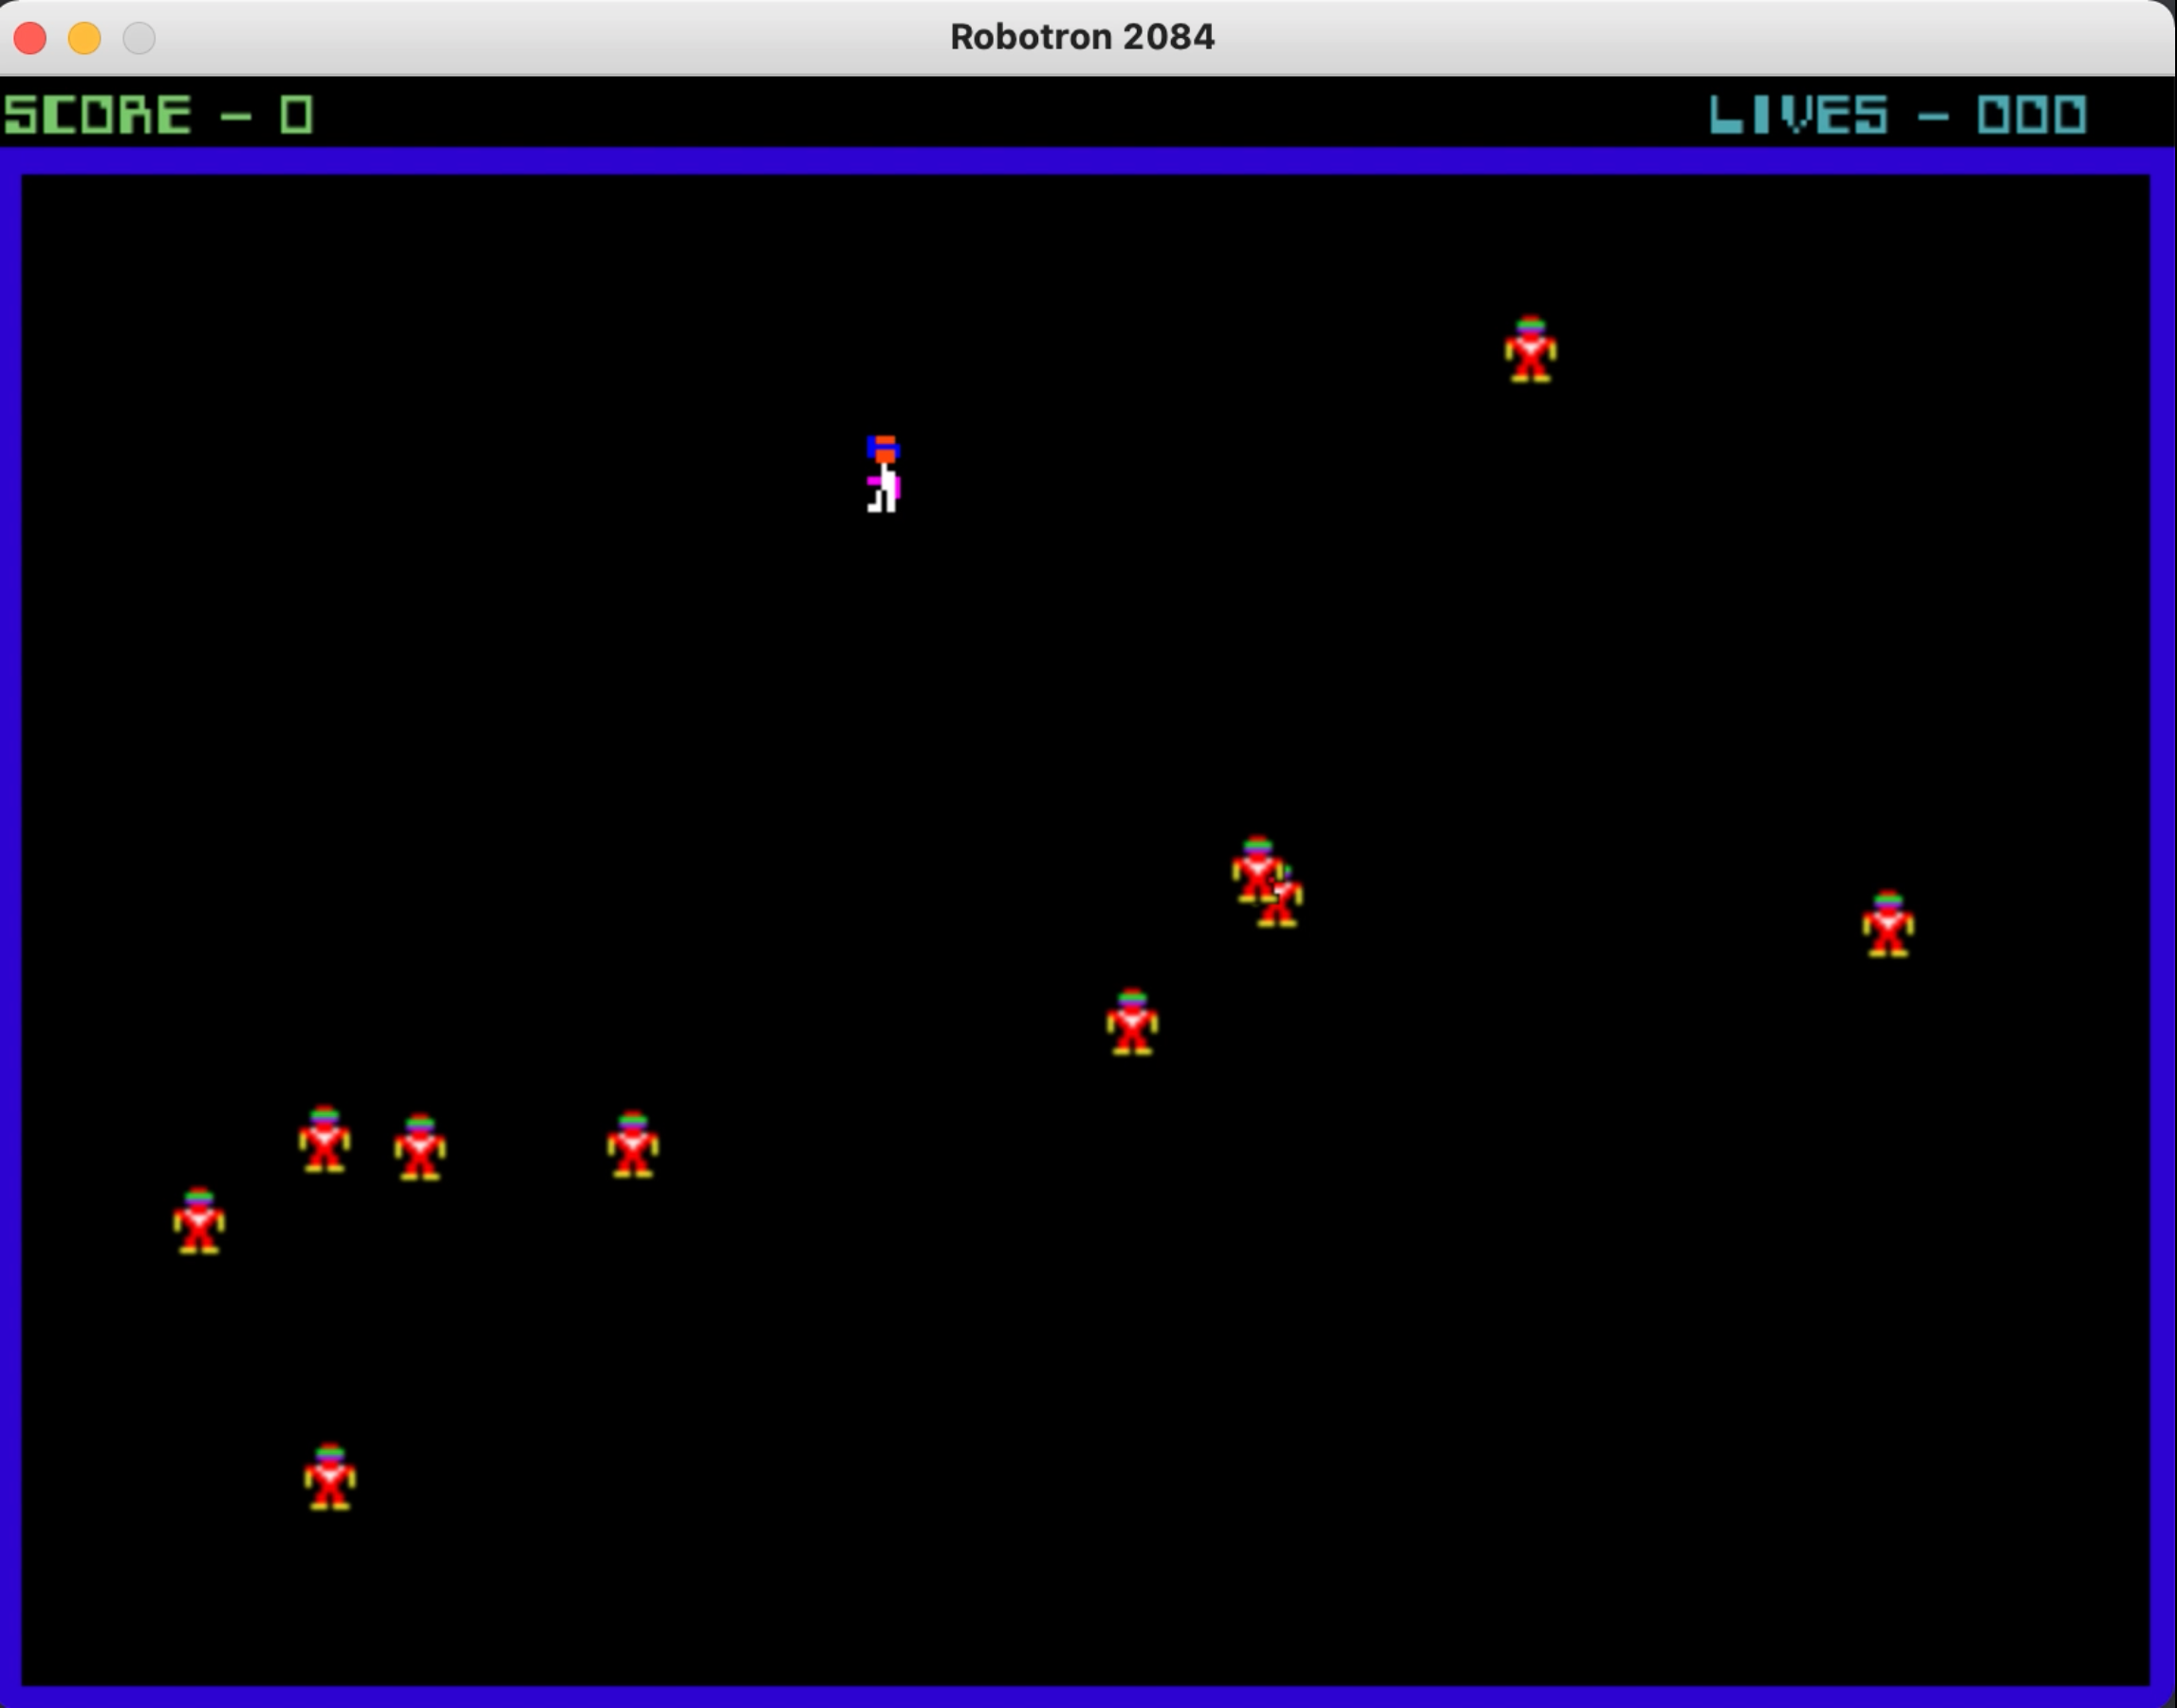
\includegraphics[width=1\linewidth]{Figures/gameplay.png}
  \centering
  \caption{Gameplay}
  \label{fig:HCI5}
\end{figure}
\newpage
This is as close as I could get to the original game, which uses a bit of a different design for the transition between levels.
\begin{figure}[H]
  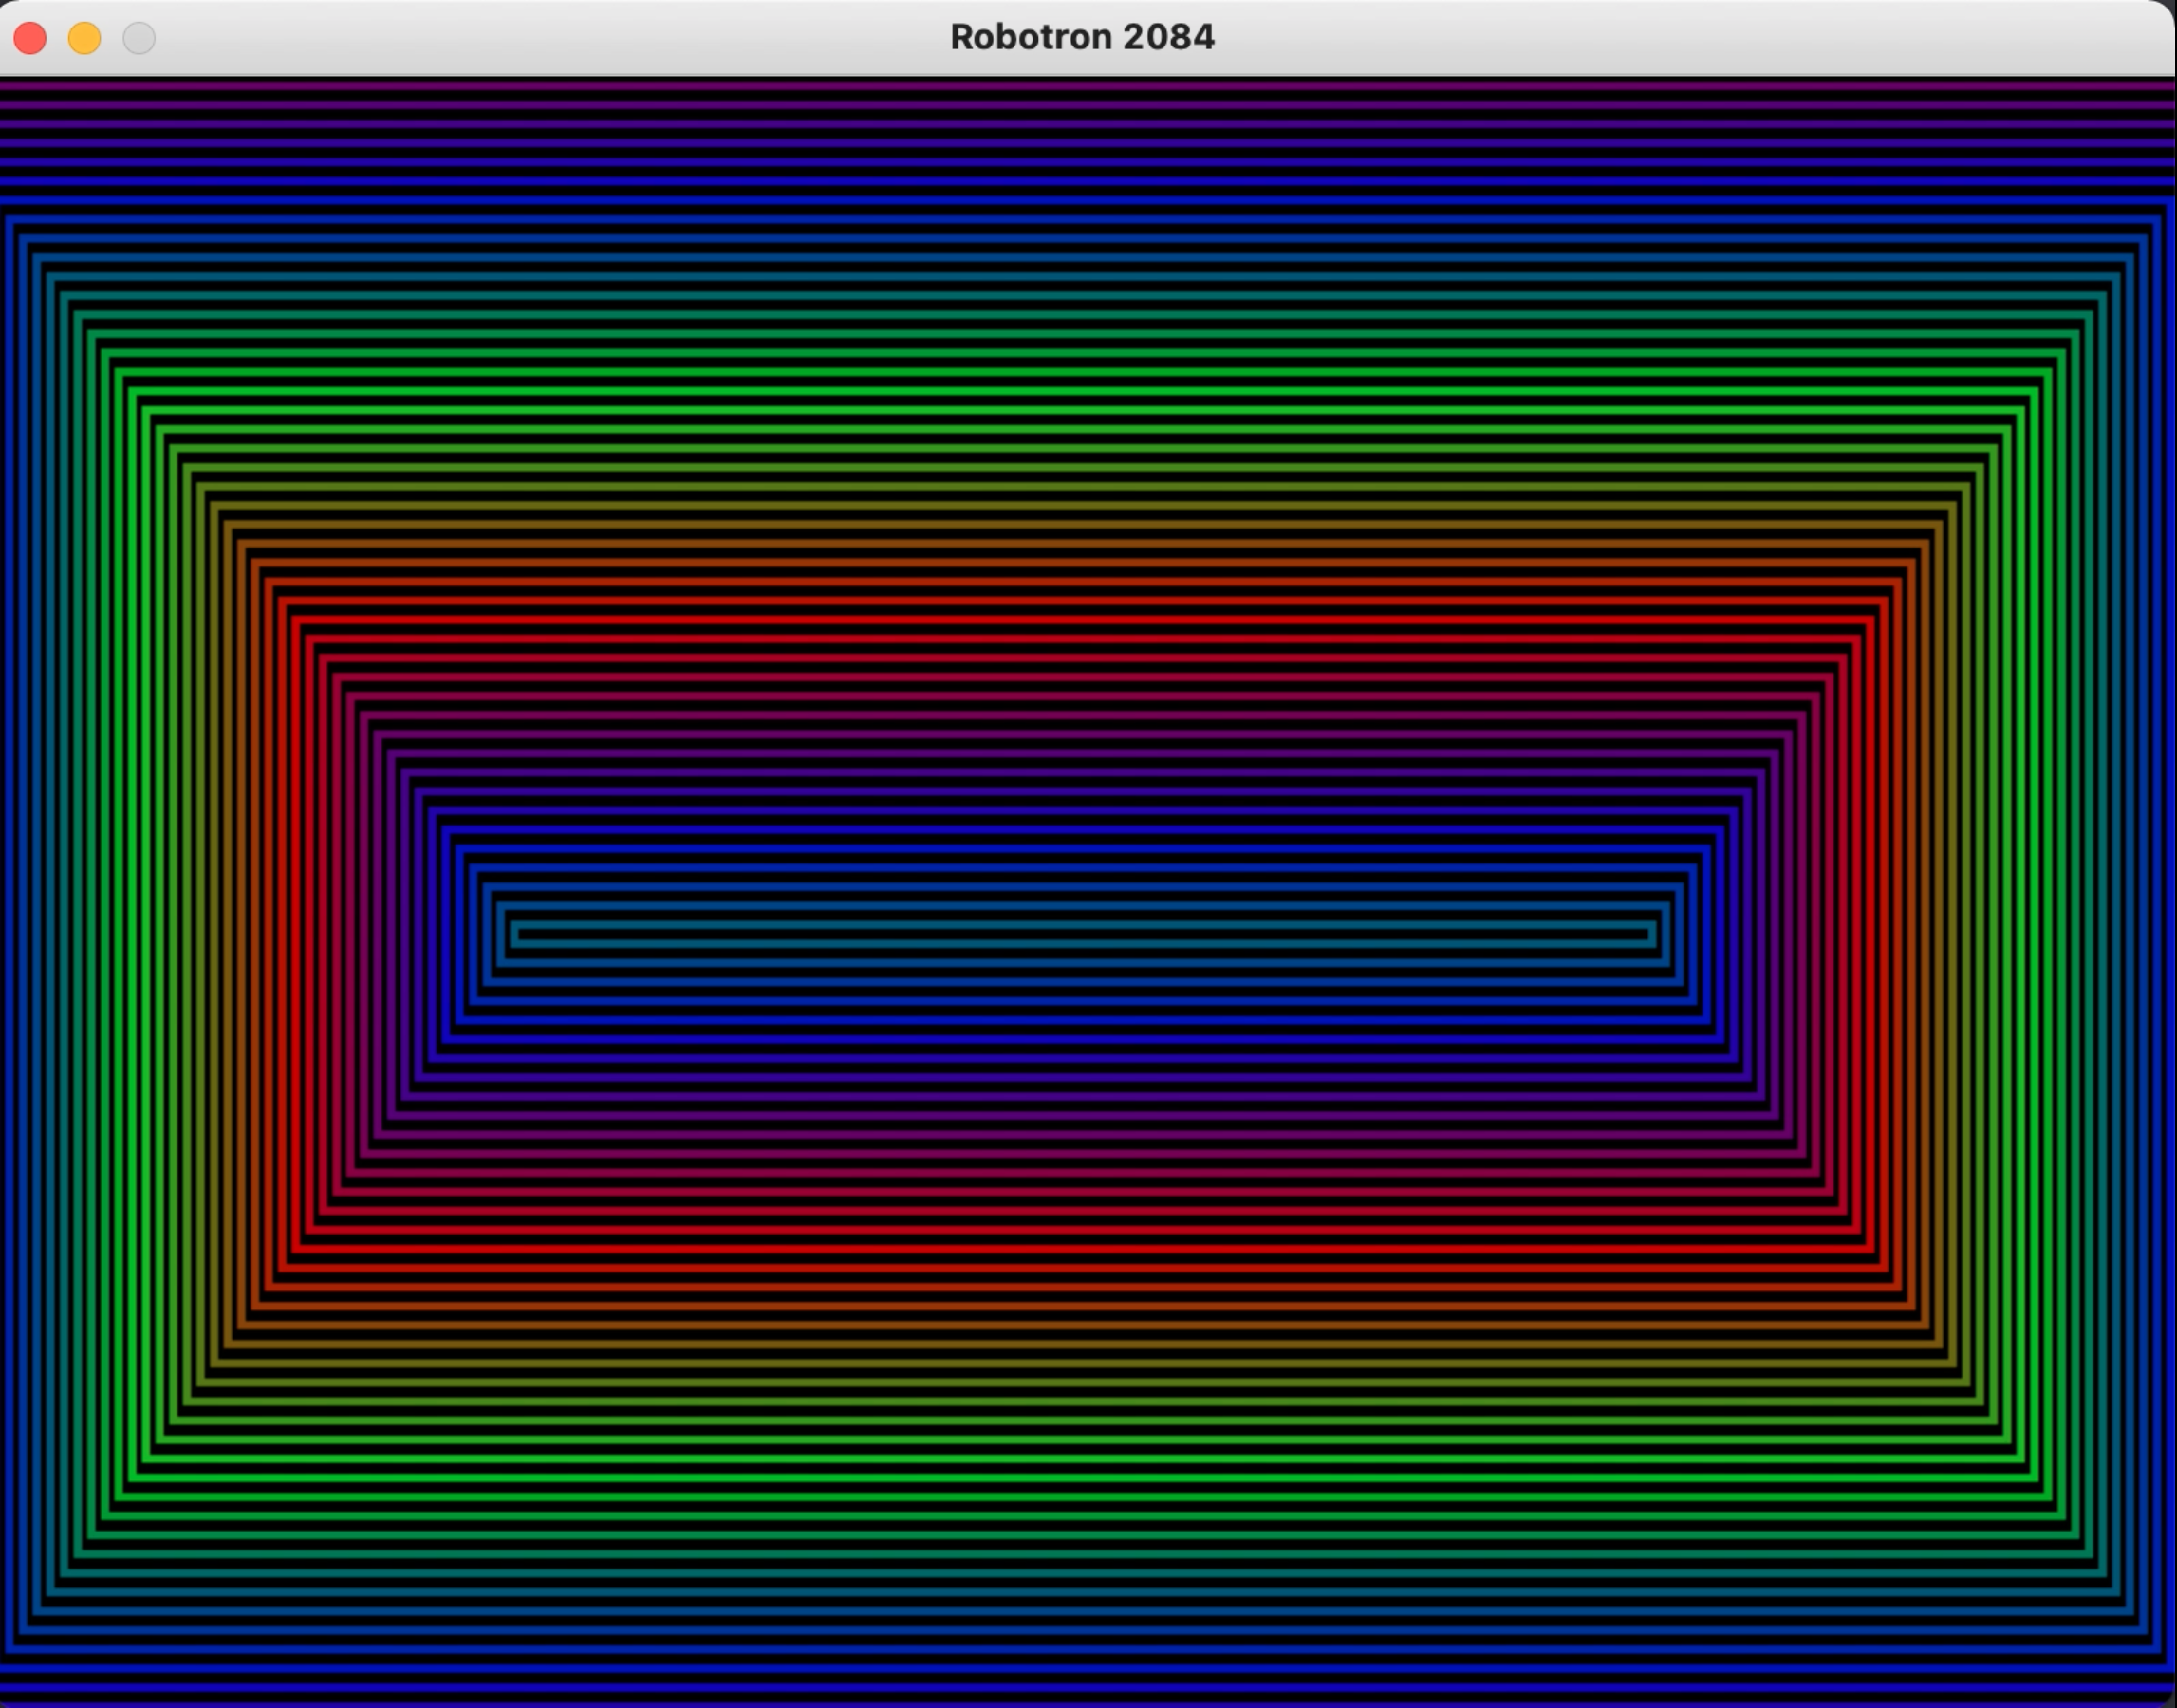
\includegraphics[width=1\linewidth]{Figures/trans.png}
  \centering
  \caption{Transition screen}
  \label{fig:HCI6}
\end{figure}

\chapter{Technical Solution}
    This chapter is split into a few sections. The first, is the file tree, and shows what all the files i use are, and how they are structured into the folder. I will then go on to show and explain some very key points in the code, however it is important to note that these snippets, as standalone code wouldnt function, as such, the content of all files of my NEA are also listed here. I will begin the sub section with all the code with a contents containing all the code listings for the NEA, and their page number, path, etc. Finally, the end of this section will be how the code is actually run. It is worth explaining, as it is not an entirely simple process.

\subsection{Folder Layout}
\dirtree{%
.1 Robotron2084.
.2 Game Code.
.3 audio.
.4 change.mp3.
.4 intro.mp3.
.4 shoot.mp3.
.3 characters\_module.
.4 \_\_init\_\_.py.
.4 characters.py.
.4 enemy.py.
.4 humans.py.
.4 player.py.
.5 sprites.py.
.3 constatnts.
.4 \_\_init\_\_.py.
.4 colors.py.
.4 const.py.
.3 controller.py.
.3 decorations.
.4 \_\_init\_\_.py.
.4 border.py.
.4 text.py
.3 event.py
.3 menu.py.
.3 model.py.
.3 objects.
.4 \_\_init\_\_.py.
.4 bullet.py.
.3 font.
.4 robotron2084.ttf.
.3 event.py.
.3 event.py.
.3 gameplay.py.
.3 main.py.
.3 sprites.
.4 2084.png.
.4 daddies.png.
.4 electrode.png.
.4 grunt.png.
.4 hulk.png.
.4 mikeys.png.
.4 mommies.png.
.4 player.png.
.3 statemachine.py.
.3 states.py.
.3 views.py.
.2 Website Code.
.3 app.py.
.3 static.
.4 css.
.5 styles.css.
.4 fonts.
.5 robotron2084.ttf.
.4 img.
.5 icon.png.
.4 js.
.5 script.min.js.
.3 templates.
.4 error.html.
.4 index.html.
.3 leaderboard.db.
.2 requirements.txt.
}

\subsection{Key Sections}
\subsubsection{Boids}
Boids was talked about in design, here is the implementation:

First step is creating the function and and setting variables
\lstinputlisting[language=Python, firstline=121, lastline=131]{"Game Code/gameplay.py"}

Now we start looping through each grunt (each member of the flock), and checking if it is 'in view' of the current (x) grunt, to do this, calculate the distance between the points and check less than 60 (eg, a grunt has a sight radius of 60) 
\lstinputlisting[language=Python, firstline=132, lastline=138]{"Game Code/gameplay.py"}

If the boid is in sight then we update our values
\lstinputlisting[language=Python, firstline=139, lastline=144]{"Game Code/gameplay.py"}

then update these values to reflect the centre of the flock etc
\lstinputlisting[language=Python, firstline=145, lastline=150]{"Game Code/gameplay.py"}

these last lines calculate and return the final v of the boid (given as $\Delta x, \Delta y$), which can be added to the current position for the new position.
\lstinputlisting[language=Python, firstline=149, lastline=155]{"Game Code/gameplay.py"}

Now we use some functional type programming to efficiently find and update all the positions
\lstinputlisting[language=Python, firstline=156, lastline=165]{"Game Code/gameplay.py"}

\subsection{stack}





\lstlistoflistings

\subsection{Website Code}

app.py
\lstinputlisting[language=Python]{"Website Code/app.py"}

index.html
\lstinputlisting[language=HTML]{"Website Code/templates/index.html"}

error.html
\lstinputlisting[language=HTML]{"Website Code/templates/error.html"}

styles.css
\lstinputlisting[language=HTML]{"Website Code/static/css/styles.css"}


\subsection{Game Code}

main.py
\lstinputlisting[language=Python]{"Game Code/main.py"}

eventmanager.py
\lstinputlisting[language=Python]{"Game Code/eventmanager.py"}

statemachine.py
\lstinputlisting[language=Python]{"Game Code/statemachine.py"}

model.py
\lstinputlisting[language=Python]{"Game Code/model.py"}

views.py
\lstinputlisting[language=Python]{"Game Code/views.py"}

controller.py
\lstinputlisting[language=Python]{"Game Code/controller.py"}

event.py
\lstinputlisting[language=Python]{"Game Code/event.py"}

states.py
\lstinputlisting[language=Python]{"Game Code/states.py"}

menu.py
\lstinputlisting[language=Python]{"Game Code/menu.py"}

gameplay.py
\lstinputlisting[language=Python]{"Game Code/gameplay.py"}

APIinteractions.py
\lstinputlisting[language=Python]{"Game Code/APIinteractions.py"}

\subsubsection{characters\_module}
characters.py
\lstinputlisting[language=Python]{"Game Code/characters_module/characters.py"}
enemy.py
\lstinputlisting[language=Python]{"Game Code/characters_module/enemy.py"}

humans.py
\lstinputlisting[language=Python]{"Game Code/characters_module/humans.py"}

player.py
\lstinputlisting[language=Python]{"Game Code/characters_module/player.py"}

sprites.py
\lstinputlisting[language=Python]{"Game Code/characters_module/sprites.py"}

\subsubsection{constants}

colors.py
\lstinputlisting[language=Python]{"Game Code/constants/colors.py"}

const.py
\lstinputlisting[language=Python]{"Game Code/constants/const.py"}

\subsubsection{decorations}
border.py
\lstinputlisting[language=Python]{"Game Code/decorations/border.py"}

\subsubsection{objects}
bullet.py
\lstinputlisting[language=Python]{"Game Code/objects/bullet.py"}

text.py
\lstinputlisting[language=Python]{"Game Code/objects/text.py"}


\chapter{Testing}
    
This section is focused mostly around the testing table below. It relies on 4 videos, uploaded to youtube, linked here:
\\
- [1] - \url{https://youtu.be/AYuTGnz5iWs}\\
- [2] - \url{https://youtu.be/YLJfJYOn0VU}\\
- [3] - \url{https://youtu.be/l1ZDcFLS0k4}\\
- [4] - \url{https://youtu.be/yuTypBxsMr4}\\

In the proof section [1] is used to denote video 1, [2] for video 2, etc, with time stamps. 

The testing shown here is only a small sample of the endless testing that went on through the iterative design process. It is worth watching the videos in their entirety to get a sense for the gameplay.
\begin{longtable}{|p{0.2\linewidth}|p{0.15\linewidth}|p{0.15\linewidth}|p{0.1\linewidth}|p{0.1\linewidth}|p{0.1\linewidth}|p{0.1\linewidth}|}
\hline
\rowcolor[HTML]{C0C0C0} 
Objective & Type of test data (Erroneous, Boundary, Normal) & Test Data & Expected Result & Actual result & Success (Y/N) & Proof \\ \hline
\endhead
%
\textbf{1 Game Tests} &  &  &  &  &  &  \\ \hline
1.1 Main (hero) character objectives &  &  &  &  &  &  \\ \hline
1.1.1 Character can be displayed & N & NA & Player gets shown & Player gets shown & Y & 0:53 - 0:57 {[}1{]} \\ \hline
1.1.2 Character can move in all 8 directions & N & W, A, S, D & Player moves in correct direction for given input & Player moves in correct direction & Y & 0:53 - 0:57 {[}1{]} \\ \hline
1.1.2 Character can move in all 8 directions & N & WA, WD, AS, SD & Player moves in correct direction for given input & Player moves in correct direction & Y & 0:06:0:10 {[}2{]} \\ \hline
1.1.3 Character faces in correct direction & N & W, S, A, D & Sprite should rotate & Sprite rotated to face correct direction & Y & 0:53 - 0:57 {[}1{]} \\ \hline
1.1.4 Characters movement is animated & N & W & Sprite should move through costumes & Sprite animated & Y & 0:53 - 0:57 {[}1{]} \\ \hline
1.1.5 Character is bounded to window & B & W, A, S, D - try to move beyond wall & Sprite shouldn’t move through the wall & Sprite is bounded to border, slightly earlier than desired & Y, but with some issue & 0:53 - 0:57 {[}1{]} \\ \hline
1.1.6 Character can shoot in 8 directions & N & W, A, S, D & Player shoots in correct direction for given input & Player shoots in correct direction & Y & 1:05 - 1:12 {[}3{]} \\ \hline
1.1.6 Character can shoot in 8 directions & N & WA, WD, AS, SD & Player shoots in correct direction for given input & Player shoots in correct direction & Y & 1:05 - 1:12 {[}3{]} \\ \hline
1.1.7 Player is invincible on load of level & B & W, A, S, D - try to run to enemy & Player doesn’t die instantly & Player doesn’t die instantly, but does die, maybe slightly too soon & Y, but with some issue & 1:18 {[}3{]} \\ \hline
1.2 Enemy character objectives (for each enemy type - Electrodes, Grunts and Hunks) &  &  &  &  &  &  \\ \hline
1.2.1 Enemies can be displayed & N & NA & Enemies shown & Enemies shown & Y & 0:53 - 0:57 {[}1{]} \\ \hline
1.2.2 Enemies can move & N & NA & Enemies move & Enemies move & Y & 0:53 - 0:57 {[}1{]} \\ \hline
1.2.3 Enemy faces correct direction & N & NA & Enemies rotate to face correct direction & Enemies rotate to face correct direction & Y & 0:10-0:15 {[}2{]} \\ \hline
1.2.4 Enemies movement is animated & N & NA & Enemies animated & Enemies animated & Y & 0:53 - 0:57 {[}1{]} \\ \hline
1.2.5 Enemy are bounded to window & N & NA & Enemies can’t walk beyond wall boundary & Enemies stopped at wall & Y & 0:15 - 0:17 {[}2{]} \\ \hline
1.2.6 Enemy kills player when touching & N & W, A, S, D into enemy & Player dies & Player dies & Y & 0:54-0:56 {[}1{]} \\ \hline
1.2.7 Specific enemy functionality &  &  &  &  &  &  \\ \hline
1.2.7.1 Electrodes are randomly spread around the page & N & NA & Electrodes are all spread out & Electrodes are all spread out & Y & 1:00 - 1:04 {[}1{]} \\ \hline
1.2.7.2 Grunts flock around player & N & W, A, S, D player tries to run away from grunt & Grunts flock towards player & Grunts flock towards player & Y & 0:50 - 1:00 {[}1{]} \\ \hline
1.2.7.3 Hunks slow down when shot & N & I, J, K, L shoot hulk, see if it slows & Hulk slows down & Hulk doesn’t noticeably down & N & 0:27-0:35 {[}2{]} \\ \hline
1.3 Menu objectives &  &  &  &  &  &  \\ \hline
1.3.1 Logo is shown and animated & N & NA & Logo animates onto screen & Logo animates onto screen & Y & 0:03 - 0:07 {[}1{]} \\ \hline
1.3.2 Display static text & N & NA & Text ends up on screen & Text ends up on screen & Y & 0:07 - 0:08 {[}1{]} \\ \hline
1.3.3 Display animated text & N & NA & Text ends up on screen & Text ends up on screen & Y & 0:07 - 0:08 {[}1{]} \\ \hline
1.3.4 Display and allow input for options & N & {[}space{]} & Will start game & Game starts & Y & 0:40-0:45 {[}1{]} \\ \hline
1.3.4 Display and allow input for options & N & {[}enter{]} & Will go to login & Login page shown & Y & 0:10-0:13 {[}1{]} \\ \hline
1.3.4 Display and allow input for options & E & {[}B{]} & Nothing happens & Nothing happened & Y & 0:10-0:11 {[}1{]} \\ \hline
1.3.4 Display and allow input for options & E & {[}a{]} & Nothing happens & Nothing happened & Y & 0:10-0:11 {[}1{]} \\ \hline
1.3.5 Allow for login and sign up & E & Sign up. Username as ‘tester123’ password as ‘password123’, ‘password’ for confirm password, ‘tes’ as initials & User not signed up, does allow sign up. Boxes go red, can’t be signed up. Incorrect message shown. & Boxes go red, can’t be signed up. Incorrect message shown. & Y & 0:10-0:15 {[}3{]} \\ \hline
1.3.5 Allow for login and sign up & N & Sign up. Username as ‘tester123’ password as ‘password123’, same for confirm password, ‘tes’ as initials & User signed up, returned to menu & User signed up, returned to menu & Y & 0:16-0:35 {[}1{]} \\ \hline
1.3.5 Allow for login and sign up & E & Log In. Username as ‘tester123’ password as ‘password12’, & User not logged in, incorrect message shown & User not logged in, incorrect message shown & Y & 0:30-0:35 {[}3{]} and 0:50-0:55 {[}3{]} \\ \hline
1.3.5 Allow for login and sign up & N & Log In. Username as ‘tester123’ password as ‘password123’, & User logged in, returned to menu & User logged in, returned to menu & Y & 0:54 - 0:58 {[}3{]} \\ \hline
1.4 Extras objectives (additional features) &  &  &  &  &  &  \\ \hline
1.4.1 Flashing border & N & NA & Border flashes & Border flashes & Y & 0:53 - 0:57 {[}1{]} \\ \hline
1.4.2 Random colour load screen & N & NA & Screen shown & Screen shown & Y & 0:00-0:02 {[}1{]} \\ \hline
1.4.3 ”All tests” screen & N & NA & Screen shown & Screen shown & Y & 0:02-0:03 {[}1{]} \\ \hline
1.4.4 Inter—level animation & N & NA & Animation shown & Animation shown & Y & 0:57-1:00 {[}1{]} \\ \hline
1.4.5 Sounds &  &  &  &  &  &  \\ \hline
1.4.5.1 For shooting & N & NA & Sound played & Sound played & Y & 1:00 - 1:04 {[}1{]} \\ \hline
1.4.5.2 For start up & N & NA & Sound played & Sound played & Y & 0:00-0:10 {[}1{]} \\ \hline
1.4.5.3 For level change & N & NA & Sound played & Sound played & Y & 0:45-0:50 {[}1{]} \\ \hline
\textbf{2 Website Tests} &  &  &  &  &  &  \\ \hline
2.1 Displays high score board of top 10 players & N & NA & Scores shown & Scores shown & Y & {[}4{]} \\ \hline
2.2 Website animated and looks like the high score board on original game & N & NA & Website is animated & Website is animated & Y & 0:03 - 0:05 {[}4{]} \\ \hline
2.3 Have an error page, informs user something went wrong & N & NA & Page shown & Page shown & Y & NA \\ \hline
2.4 API Goals (a route to...) &  &  &  &  &  &  \\ \hline
2.4.1 Return top scores & N & NA & Returned & Returned & Y & NA \\ \hline
2.4.2 Allow for sign up & N & “test12345”, “password123”, “JAM” & Return ‘success’ & Return ‘success’ & Y & NA \\ \hline
2.4.3 Allow for log in & N & “test12345”, “password123” & Return token & Return token & Y & NA \\ \hline
2.4.3 Allow for log in & E & “test12345”, “password13” & Return password error & Return password error & Y & NA \\ \hline
2.4.4 Generate tokens for login & N & “test12345”, “password123” & Return token & Return token & Y & NA \\ \hline
2.4.4 Generate tokens for login & E & “test12345”, “password13” & Return password error & Return password error & Y & NA \\ \hline
2.4.5 Upload scores and validate with token & N & userID, “2000”, token & Return ‘success’ & Return ‘success’ & Y & NA \\ \hline
2.4.5 Upload scores and validate with token & E & userID, “2000”, ‘1’ (incorrect token) & Return password error & Return password error & Y & NA \\ \hline
\end{longtable}
\chapter{Evaluation}
    
Overall, I think I was very successful in my project. I worked on it over the space of many months, and am very proud of the result. I think it is probably my favourite project, it has allowed me to discover many new technologies, approaches and methods. I have not only enjoyed working on it, but think that the end result almost perfectly matches what I wanted originally. Having spoken to 2 reviewers, I have found that other people also agree. \\

One student enjoyed the game, commenting on how it was very fast paced, and thought the implementation was perfect. The possible improvement comment was to add different difficulty levels, thinking about this, i can think of a few possible implementations. One would be to view the levels.csv as a ratio of enemies, more than a definite number. With this, with this, a difficulty multiplier could be used to set the difficulty. However, I think there is a better solution: Have multiple CSV's, and also have different constants, allowing, for example, grunts to move faster. This means there can be lots of variation in difficulties, and lots of different settings. I really like the idea of implementing this - and plan on doing it in the future.\\

Another student had similar ideas, but also thought an improvement would be to use a controller to allow the dual stick shooter to really come to life. This is somewhat simple on the surface, as pygame has a feature to allow this, so it would be a great demonstration of the MVC's modularity. The also has some further details, as it would allow me to move in more than 8 directions - i could move (and shoot) in the true angle of the stick. This bring some complexity with the fact that the velocity still needs to be a constant, so would require lots more trigonometry to calculate a xy movement vector.\\

This table of objectives shows how well i managed to meet all the objectives that were set for the project.
\begin{longtable}{|p{0.3\linewidth}|p{0.1\linewidth}|p{0.6\linewidth}|}
\hline
\rowcolor[HTML]{C0C0C0} 
Objective & Met? & Comments \\ \hline
\endhead
%
{\ul \textbf{1 Game Objectives}} &  &  \\ \hline
\textbf{1.1 Main (hero) character objectives} &  &  \\ \hline
1.1.1 Character can be displayed & Y & Player is shown, this one was quite simple \\ \hline
1.1.2 Character can move in all 8 directions & Y & Yes, this works, player moves with WASD, holding 2 will allow the player to move diagonally \\ \hline
1.1.3 Character faces in correct direction & Y & As a player presses a WASD key the direction the sprite faces is changed as required. \\ \hline
1.1.4 Characters movement is animated & Y & As a player moves, they "walk" \\ \hline
1.1.5 Character is bounded to window & Y & Player can't move outside of the window, probably could have allowed them to get closer to the border though \\ \hline
1.1.6 Character can shoot in 8 directions & Y & IJKL, and like moving, holding 2 goes in the diagonal \\ \hline
1.1.7 Player is invincible on load of level & Y & Player gets a few ticks of invincibility \\ \hline
\textbf{1.2 Enemy character objectives (for each enemy type - Electrodes, Grunts and Hunks)} &  &  \\ \hline
1.2.1 Enemies can be displayed & Y & Enemies are displayed, based on the amount in the levels.csv file \\ \hline
1.2.2 Enemies can move & Y & Enemies have an interface which can be used to move them \\ \hline
1.2.3 Enemy faces correct direction & Y & Every tick updates the direction, ensures they face in the correct direction. works as expected, could however have added a way for them to move diagonally and animate that way (for now just faces either way) \\ \hline
1.2.4 Enemies movement is animated & Y & Yes, grunts and hulks animate as they walk \\ \hline
1.2.5 Enemy are bounded to window & Y & Just like players, these could have pushed closer to the window border I guess \\ \hline
1.2.6 Enemy kills player when touching & Y & Players die from touching the bounding box yes, however for electrodes this is kind of an issue, as they aren't a box shape - there wasn't an easy fix for this. \\ \hline
\textbf{1.2.7 Specific enemy functionality} &  &  \\ \hline
1.2.7.1 Electrodes are randomly spread around the page & Y & Uses random numbers to spread them, could have used a generator which forces more of an even distribution, but they end up quite well distributed anyway. \\ \hline
1.2.7.2 Grunts flock around player & Y & Implementation of this isn't ideal but works well enough for this project. If I had wanted to add some more complexity, it would have been interesting to use a "sight" which will only allow the grunt to see within a certain space - so if the player was out of range they would be unable to move to them, for example. \\ \hline
1.2.7.3 Hunks slow down when shot & Y & Hunks have 2 speeds, and whilst they are shot they have an attribute changed so they move at a slower rate. \\ \hline
\textbf{1.3 Menu objectives} &  &  \\ \hline
1.3.1 Logo is shown and animated & Y & Logo animates, close to how the original did, but would have looked better sliced up and moving as a "wave" - rather than linearly shrinking. \\ \hline
1.3.2 Display static text & Y & All text is shown, and rather well in terms of the implementation \\ \hline
1.3.3 Display animated text & Y & The flashing text flashes as I wanted it to, using random colours \\ \hline
1.3.4 Display and allow input for options & Y & By pressing keys and using the mouse, the user can input into the program. \\ \hline
1.3.5 Allow for login and sign up & Y & Users login and sign up, and a token is stored to maintain the log in when the program is stopped. \\ \hline
\textbf{1.4 Extras objectives (additional features)} &  &  \\ \hline
1.4.1 Flashing border & Y & Border flashes random colours around the screen - I even implemented a score and life counter on this \\ \hline
1.4.2 Random colour load screen & Y & This is the first screen shown, random coloured squares, hard to make it wrong \\ \hline
1.4.3 ”All tests” screen & Y & Again, a really basic screen \\ \hline
1.4.4 Inter—level animation & Y & Not as close to the original game as I would have liked, but looks cool none the less \\ \hline
\textbf{1.4.5 Sounds} &  &  \\ \hline
1.4.5.1 For shooting & Y & Taken and isolated as well as possible \\ \hline
1.4.5.2 For start up & Y & Taken and isolated as well as possible \\ \hline
1.4.5.3 For level change & Y & Taken and isolated as well as possible \\ \hline
{\ul \textbf{2 Website Objectives}} &  &  \\ \hline
2.1 Displays high score board of top 10 players & Y & Shows the scores \\ \hline
2.2 Website animated and looks like the high score board on original game & Y & Animates on load, window border flashes up \\ \hline
2.3 Have an error page, informs user something went wrong & Y & On a 500 error, the error page shows saying that something went wrong \\ \hline
\textbf{2.4 API Goals (a route to...)} &  &  \\ \hline
2.4.1 Return top scores & Y & This API didn't end up being used, but was still implemented none the less \\ \hline
2.4.2 Allow for sign up & Y & API route works perfectly, returns errors when needed \\ \hline
2.4.3 Allow for log in & Y & API route works perfectly, returns errors when needed \\ \hline
2.4.4 Generate tokens for login & Y & Tokens are easily generated and stored on the client \\ \hline
2.4.5 Upload scores and validate with token & Y & Score uploading works as hoped, is perfect, uses tokens to validate, so no need to log in or sign up \\ \hline
\end{longtable}

To conclude, working on this project has been months of work, but is very much concluding here. After all the work it is very rewarding to be able to look back on the year of work put into it, and the result is ideal and exactly what I had hoped for, back when I started it. I met all the objectives set, and whilst the system could be improved, for example, by allowing for a better connected API (allowing users to look up a database of scores and results for example). As such I would deem the project a success, and thank the reader for taking the time to read my report into it.

\begin{figure}[H]
    
  
\includegraphics[width=.4\textwidth,right]{Figures/sign.png}
  
\end{figure}
\end{document}

\end